\chapter{Recurrent Neural Networks}
\section{Feed-Forward Neural Networks vs Recurrent Neural Networks}

\begin{itemize}
    \item Feed-Forward Neural Networks (FFNNs) are the simplest type of artificial neural network architecture. In a FFNN, information moves in only one direction—forward—from the input nodes, through the hidden nodes (if any), and finally to the output nodes. There are no cycles or loops in the network.
    
    \item Recurrent Neural Networks (RNNs), on the other hand, have connections that form directed cycles. This means that information can be recycled in the network, allowing them to maintain a `memory' of previous inputs. This is particularly useful for tasks that require the network to remember across time steps, like language modelling and time series prediction.
    
    \item The main architectural difference is that RNNs have a recurrent hidden state whose activation at each time is dependent on that of the previous time step, which is not the case for FFNNs.
\end{itemize}
\begin{figure}[H]
    \centering
    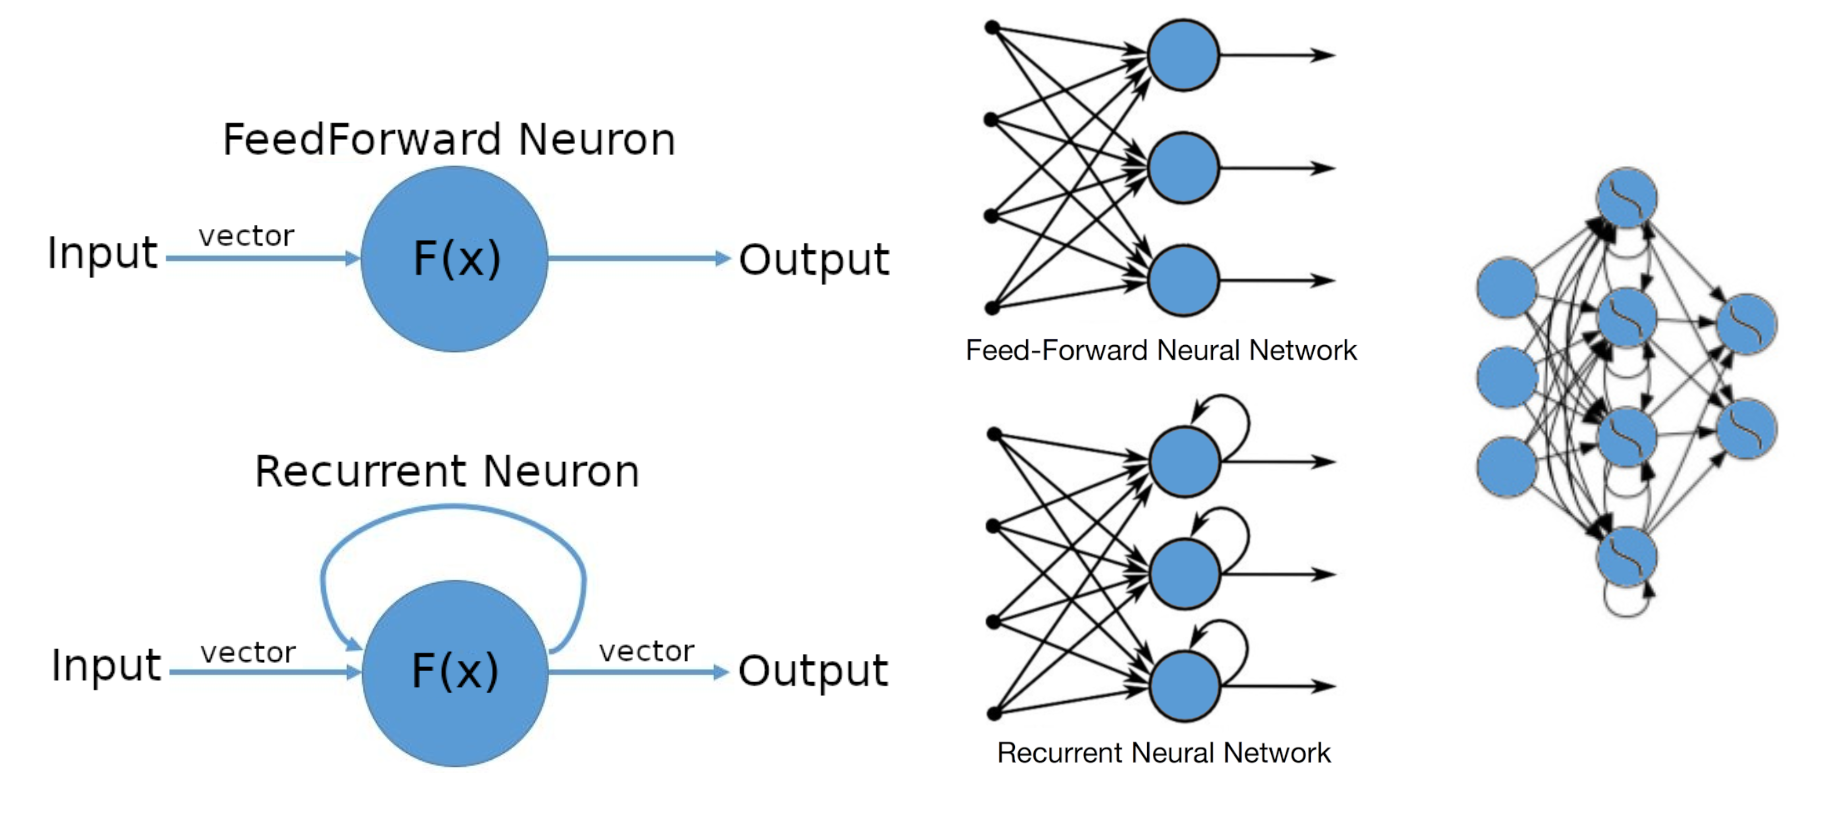
\includegraphics[width=0.75\linewidth]{img/ffnn_vs_rnn.png}
\end{figure}

\section{Structure of RNNs}
\begin{itemize}
    \item Recurrent Neural Networks (RNNs) exhibit a chain-like structure, making them particularly suitable for processing sequences and lists such as speech, language, text, and temporal data like audio and video streams.
    \item The architecture of RNNs allows for the handling of input and output sequences of variable lengths, a feature that is leveraged in applications such as dialog generation.
    \item In dialog generation, for instance, RNNs can be used to generate a response based on an input question. The process involves encoding the semantic meaning of words into numerical embeddings which the network uses to understand context and generate appropriate answers.
    \item The use of softmax functions at each output stage in sequence models like RNNs helps in generating suggestions or predictions for the next word in a sequence, enabling applications such as text auto-completion and machine translation.
\end{itemize}
\begin{figure}[H]
    \centering
    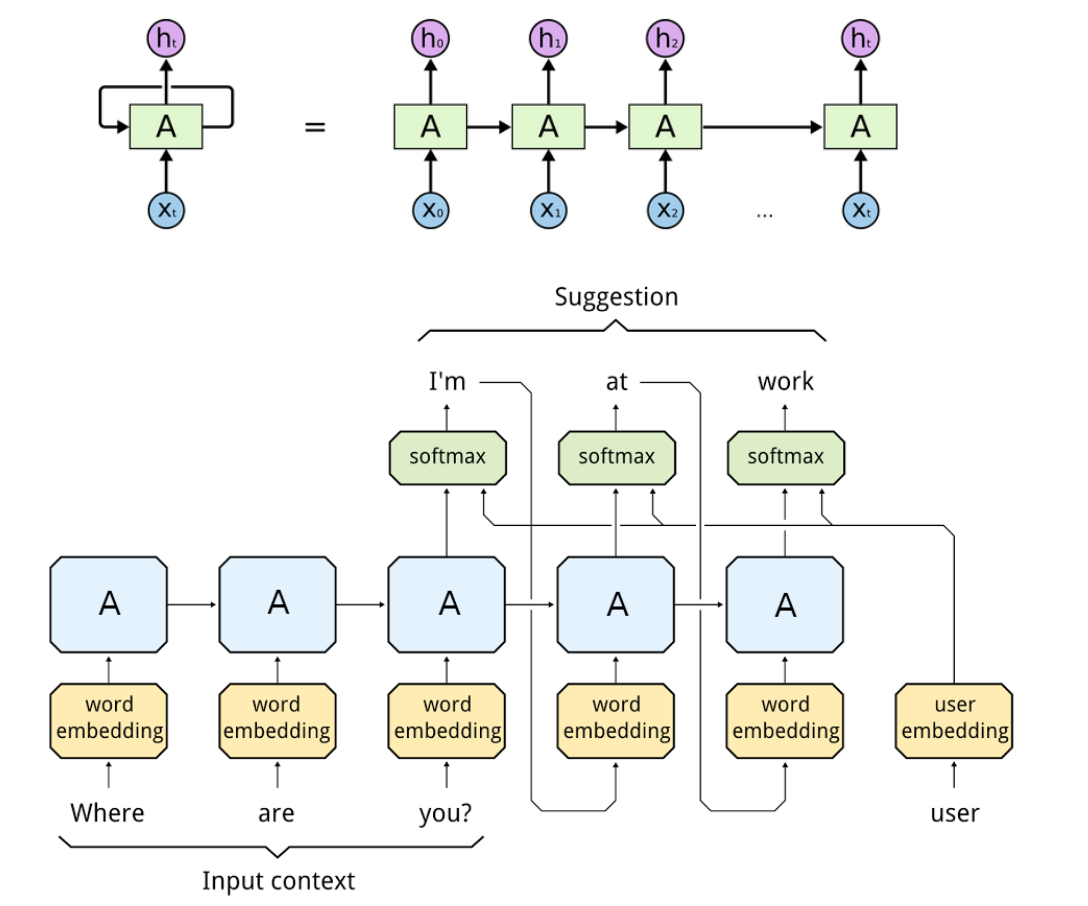
\includegraphics[width=0.5\linewidth]{img/rnn_structure.png}
    
\end{figure}


\subsection{Word Embeddings}
\begin{itemize}
    \item Word embedding is a real number-vector numerical representation of a word or text.
    \item Words with similar meanings will be closer together in the embedding space of vectors. This is to capture a sort of relationship within that space, e.g. meaning, morphology, context, etc.
\end{itemize}
\begin{figure}[H]
\begin{center}
\begin{tikzpicture}
    \begin{axis}[
        xmin=-10, xmax=10,
        ymin=-1, ymax=7,
        axis lines=middle,
        axis line style={->},
        xlabel={$x$},
        ylabel={$y$},
        xtick={-10,-9,...,10},
        ytick={-1,0,...,7},
        xticklabels={,,},
        yticklabels={,,},
        xlabel style={at={(ticklabel* cs:1)},anchor=north west},
        ylabel style={at={(ticklabel* cs:1)},anchor=south west}
    ]
    \tikzset{>=Latex} % correct this line by removing the space

    % Vector arrows
    \draw[->,red] (axis cs:0,0) -- (axis cs:3,6) node[midway, above left] {King};
    \draw[->,teal] (axis cs:0,0) -- (axis cs:4,5) node[midway, above] {Queen};
    \draw[->,red] (axis cs:0,0) -- (axis cs:6,3) node[midway, below] {Man};
    \draw[->,teal] (axis cs:0,0) -- (axis cs:8,1) node[end, below] {Woman};

    % King - Man vector
    \draw[->, orange] (axis cs:0,0) -- (axis cs:-3,3) node[midway, below left] {King$-$Man};

    % Queen - Woman vector
    \draw[->, orange] (axis cs:0,0) -- (axis cs:-4,4) node[midway, below left] {Queen$-$Woman};
    \end{axis}
\end{tikzpicture}
\end{center}
\end{figure}

\begin{itemize}
    \item \textbf{One-Hot Encoding (Count Vectoring)} involves creating a binary vector for each word in the vocabulary with a 1 indicating the presence of the word in a given document and 0 indicating its absence. 
    \begin{itemize}
        \item \textbf{Example:} Given the vocabulary \{Rome, Paris, Italy, France\}, the sentence "Rome and Italy" would be vectorised as [1, 0, 1, 0]. Different lengths of sentences will still have the same length vector.
        \item \textbf{Example:} Given the vocabulary \{Rome, Paris, Italy, France\}, the sentence "I like Rome, not just Rome but Italy" would be vectorised as [1, 0, 1, 0]. 
        \item Note that it captures the words, but ignores the semantic relationship, nor its similarity or contextual meaning.
    \end{itemize}

    \item \textbf{Bag of Words} is a representation of text that describes the presence of words within a document but . It's often used in conjunction with methods like TF-IDF. It is similar to One-Hot encoding, but also keeps track of the number of occurences. 
    \begin{itemize}
        \item \textbf{Example:} Given the vocabulary \{Rome, Paris, Italy, France\}, the sentence "I like Rome, not just Rome but Italy" would be vectorised as [2, 0, 1, 0].  
        \item It does not consider the order of words.
        \item \textbf{Example:} The sentences ``Rome is a city" and``Is Rome a city?" would have the same Bag of Words representation if order is not considered.
    \end{itemize}

    \item \textbf{TF-IDF (Term Frequency-Inverse Document Frequency)} vectors weigh the frequency of a word in a document against its frequency across all documents, diminishing the importance of words that occur very frequently across documents (such as `the', `is', `and').
    \begin{itemize}
        \item \textbf{Example:} If the word ``Rome" appears often in one document but rarely in others, it will have a high TF-IDF score in that particular document.
        \item \textbf{Example: } Consider the corpus: \\
        ``I love this movie”,
        ``This movie is terrible”,
        ``The plot is confusing”\\
        \[
\begin{array}{c|cccccccc}
& \text{confusing} & \text{is} & \text{love} & \text{movie} & \text{plot} & \text{terrible} & \text{the} & \text{this} \\
\hline
\text{Document 1} & 0 & 0 & 0.51 & 0.77 & 0 & 0 & 0 & 0.39 \\
\text{Document 2} & 0 & 0.46 & 0 & 0.46 & 0 & 0.60 & 0 & 0.46 \\
\text{Document 3} & 0.53 & 0.40 & 0 & 0 & 0.53 & 0 & 0.53 & 0 \\
\end{array}
\]
        

        
    \end{itemize}

    \item \textbf{Co-occurrence Matrix} represents how often words appear together in a context within a given corpus. The matrix has a size of $V \times V$, where $V$ is the vocabulary size, and the entry at row $i$, column $j$ indicates how often the $i$-th word occurs with the $j$-th word.
    
    \begin{itemize}
        \item \textbf{Example:} In a simple corpus, the word "deep" might often occur with "learning" and less frequently with "flying", resulting in higher counts in the corresponding entries of the matrix.\\
         \[
        \begin{array}{c|cccccccc}
         & \text{I} & \text{like} & \text{enjoy} & \text{deep} & \text{learning} & \text{NLP} & \text{flying} & \text{.} \\
        \hline
        \text{I} & 0 & 2 & 1 & 0 & 0 & 0 & 0 & 0 \\
        \text{like} & 2 & 0 & 0 & 1 & 0 & 1 & 0 & 0 \\
        \text{enjoy} & 1 & 0 & 0 & 0 & 0 & 0 & 1 & 0 \\
        \text{deep} & 0 & 1 & 0 & 0 & 1 & 0 & 0 & 0 \\
        \text{learning} & 0 & 0 & 0 & 1 & 0 & 0 & 0 & 1 \\
        \text{NLP} & 0 & 1 & 0 & 0 & 0 & 0 & 0 & 1 \\
        \text{flying} & 0 & 0 & 1 & 0 & 0 & 0 & 0 & 1 \\
        \text{.} & 0 & 0 & 0 & 0 & 1 & 1 & 1 & 0 \\
\end{array}
        \]
    \end{itemize}

    \item \textbf{Word2Vec and Doc2Vec}
        \begin{itemize}
        \item Both forms utilise a shallow neural network architecture trained on large corpora to detect word usage patterns.
        \item The model effectively captures semantic relationships between words, allowing for operations like vector addition and subtraction to reveal analogous relationships.
        \item Word2Vec accounts for single-word contexts whereas Doc2Vec extends to multi-word document contexts, encapsulating more complex structures.
    \end{itemize}
    \begin{figure}[H]
        \centering
        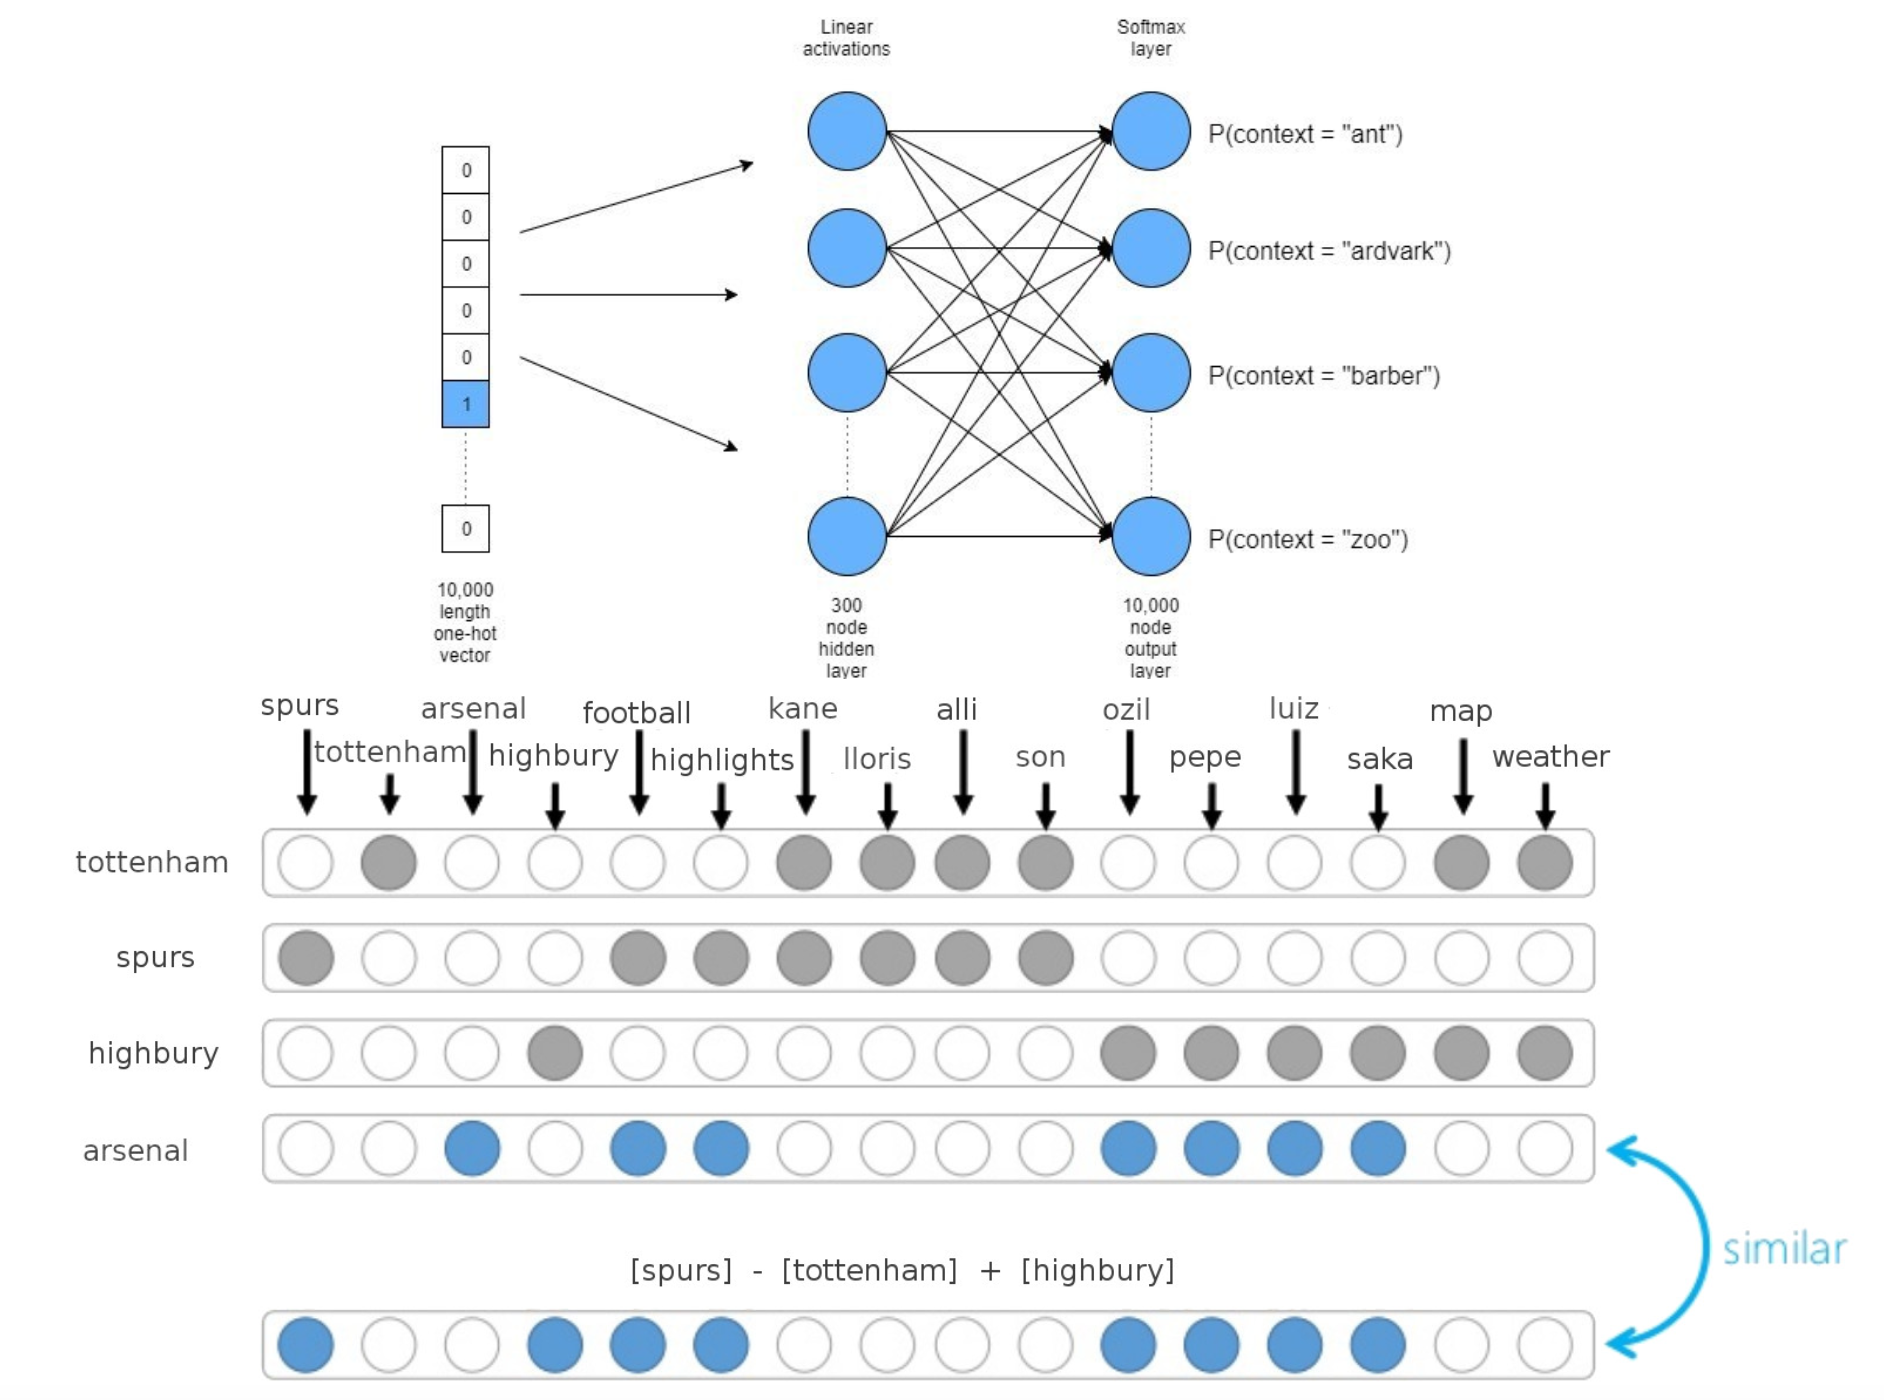
\includegraphics[width=0.75\linewidth]{img/w2v.png}
    \end{figure}

    \item \textbf{GloVe Embeddings: } GloVE, short for (Global Vectors for Word Representation) is an unsupervised learning algorithm for generating word embeddings.
    \begin{itemize}
        \item It uses global matrix factorisation techniques with a local context window to balance the focus between global statistics and local word co-occurrence.
        \item This helps GloVe capture both linear substructures and the semantics of word-word relationships within the corpus.
    \end{itemize}
    \begin{figure}[H]
        \centering
        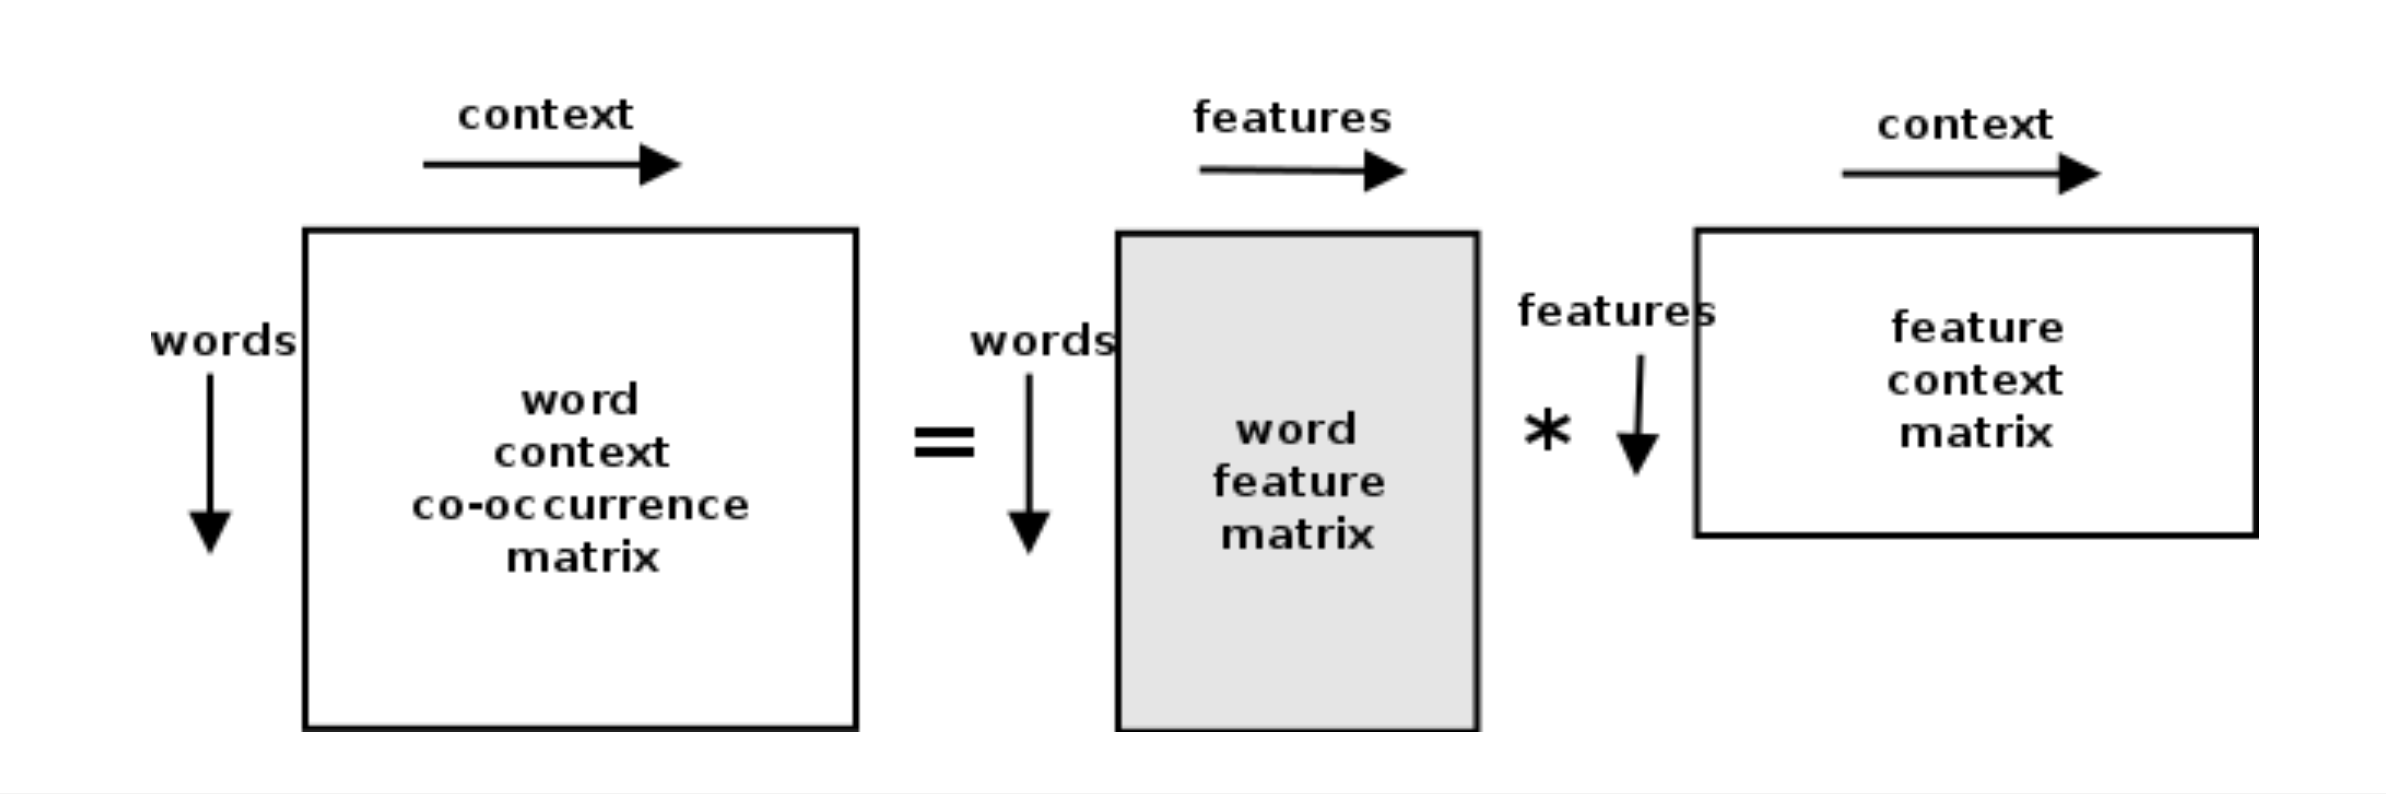
\includegraphics[width=0.75\linewidth]{img/glove.png}
        
    \end{figure}
\end{itemize}

\subsection{RNN Unit}
\begin{itemize}
    \item RNNs handle inputs $x_t \in \mathbb{R}^{N_{in}}$ and produce outputs $y_t \in \mathbb{R}^{N_{out}}$ for each timestep $t$.
    \item RNNs utilise a distributed hidden state, allowing them to store and process sequential information over time.
    \item They can be viewed as layered, feedforward networks with shared weights across the timesteps, which are trained using backpropagation through time (BPTT).
    \item During BPTT, gradients from all timesteps are accumulated for each weight, accounting for the shared weight structure.
    \item The hidden state $h_t \in \mathbb{R}^{N_h}$ is updated at each timestep according to:
    \begin{equation}
    h_t = \theta(W^{(hh)} h_{t-1} + W^{(xh)} x_t + b_h)
    \end{equation}
    where $\theta$ is a nonlinear activation function such as $\tanh$.
    \item The output $y_t$ is given by:
    \begin{equation}
    y_t = W^{(hy)} h_t + b_y
    \end{equation}
    with weight matrices:
    \begin{itemize}
        \item $W^{(hh)} \in \mathbb{R}^{N_h \times N_h}$
        \item $W^{(xh)} \in \mathbb{R}^{N_h \times N_{in}}$
        \item $W^{(hy)} \in \mathbb{R}^{N_{out} \times N_h}$
    \end{itemize}  and bias terms $b_h \in \mathbb{R}^{N_h}$, $b_y \in \mathbb{R}^{N_{out}}$.
    \item Outputs can also be fed back into the network as inputs for subsequent timesteps, e.g., $x_{t+1} = y_t$, to create a sequence-to-sequence model.
\end{itemize}

\begin{figure}[ht]
    \centering
    \begin{subfigure}[b]{0.4\textwidth}
        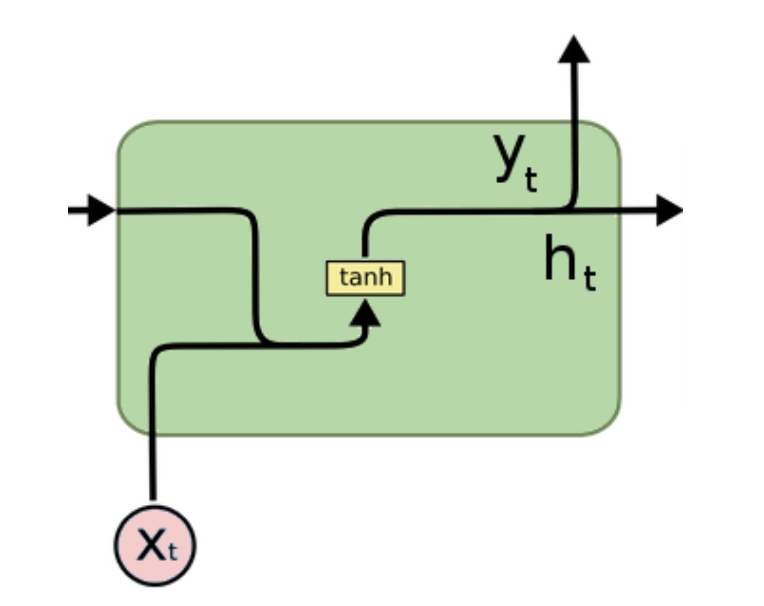
\includegraphics[width=\linewidth]{img/RNN_unit.png}
        \caption{A single RNN unit}
    \end{subfigure}
    \begin{subfigure}[b]{0.5\textwidth}
        \includegraphics[width=\linewidth]{img/RNN_structure.png}
        \caption{An RNN structure}
    \end{subfigure}
\end{figure}

\begin{itemize}

    \item RNNs are well-suited for modelling short-term dependencies due to the recurrent connections between hidden states.
    \item However, they often struggle with long-term dependencies because of the vanishing gradient problem, where gradients can become exponentially small as they propagate back through timesteps, leading to minimal weight updates and poor learning of long-range dependencies.
    \begin{equation}
        \delta^{(I)}=\left(\prod_{k=I}^{L-1}\theta^{\prime}(s^{(k)})(W^{(k)})^T\right)\theta^{\prime}(s^{(L)})\nabla_{x^{(L)}}\mathcal{L}
    \end{equation}
\end{itemize}


\begin{figure}[H]
    \centering
    

\end{figure}
\break
\subsection{Long Short Term Memory}
LSTM units are designed to address the long-term dependency problem present in traditional RNNs by incorporating mechanisms that allow for preserving information over extended periods.
\begin{figure}[H]
    \centering
    \begin{subfigure}[b]{0.45\textwidth}
        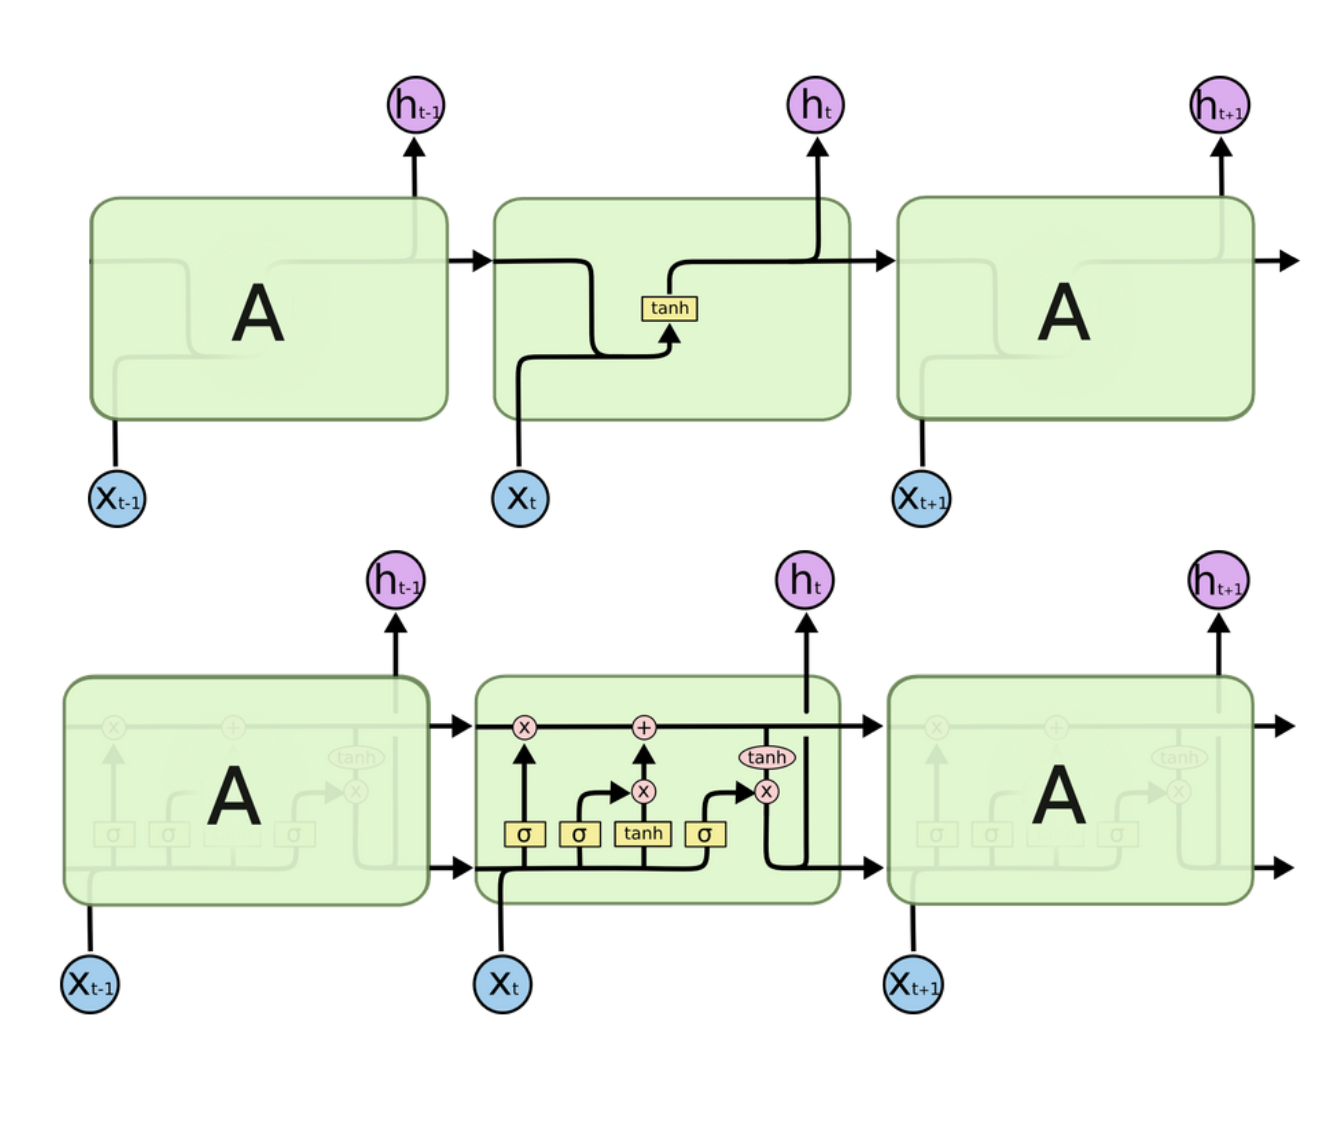
\includegraphics[width=\linewidth]{img/LSTM.png}
        \caption{LSTM units diagram}
    \end{subfigure}
    \begin{subfigure}[b]{0.30\textwidth}
        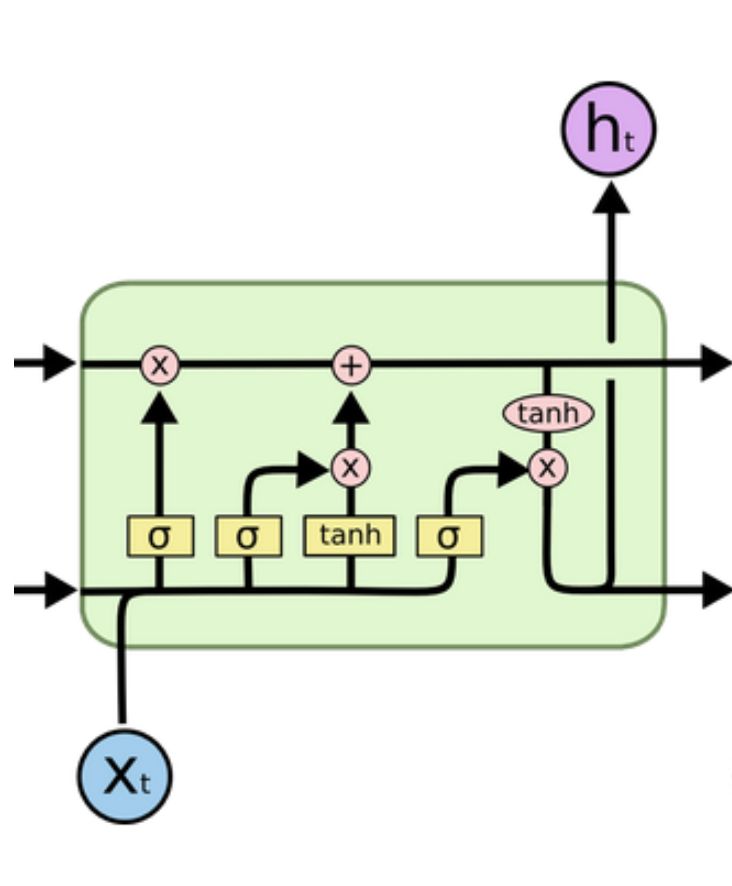
\includegraphics[width=\linewidth]{img/LSTM_closeup.png}
        \caption{LSTM unit close-up}
    \end{subfigure}
\end{figure}

\begin{figure}[H]
    \centering
    \begin{subfigure}[b]{0.4\textwidth}
        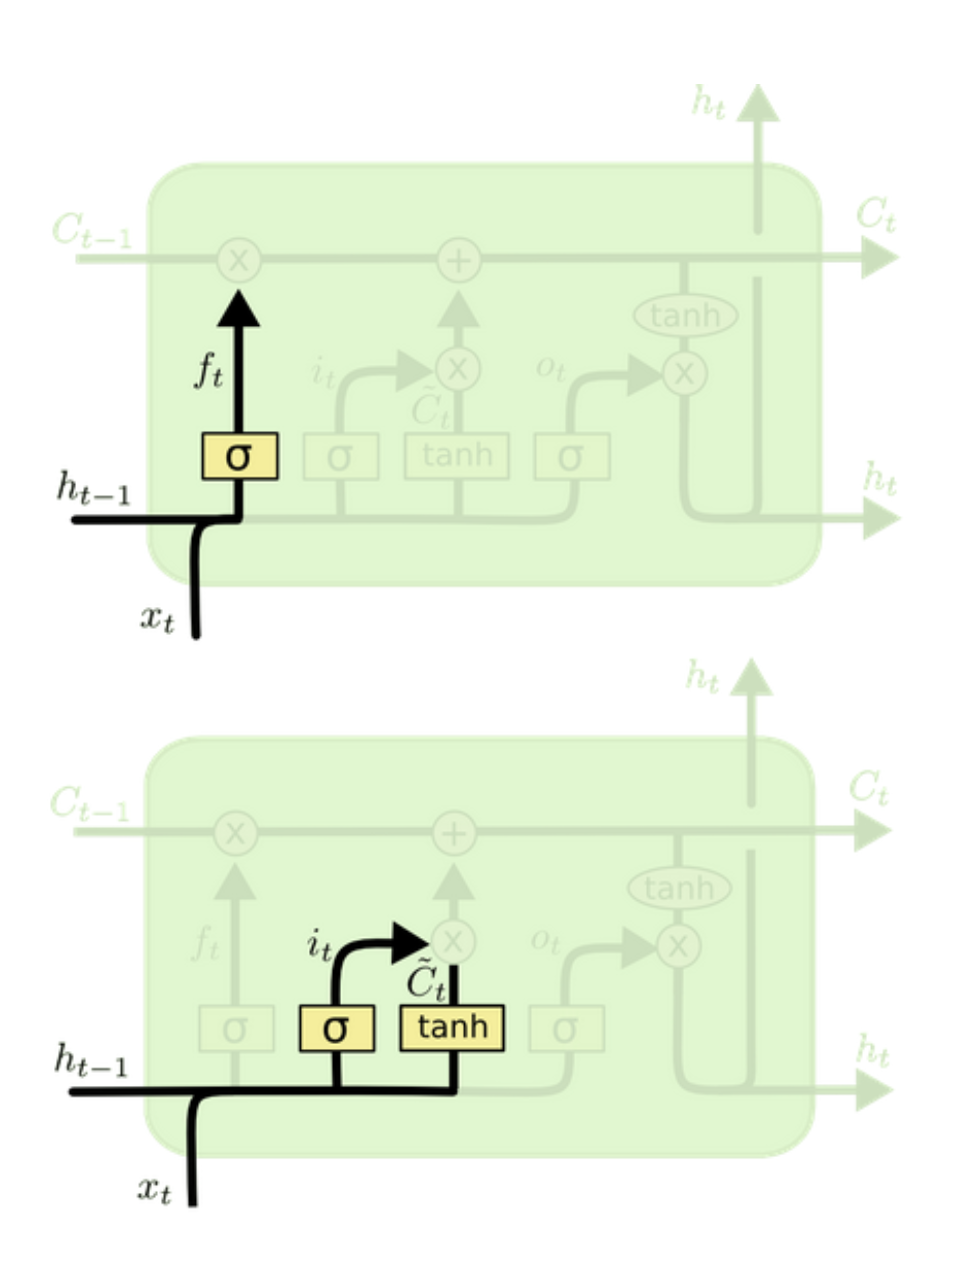
\includegraphics[width=\linewidth]{img/LSTM_unit.png}
        \caption{Forget Gate $f_t$ and Update Gate $i_t$}
    \end{subfigure}
    \begin{subfigure}[b]{0.4\textwidth}
        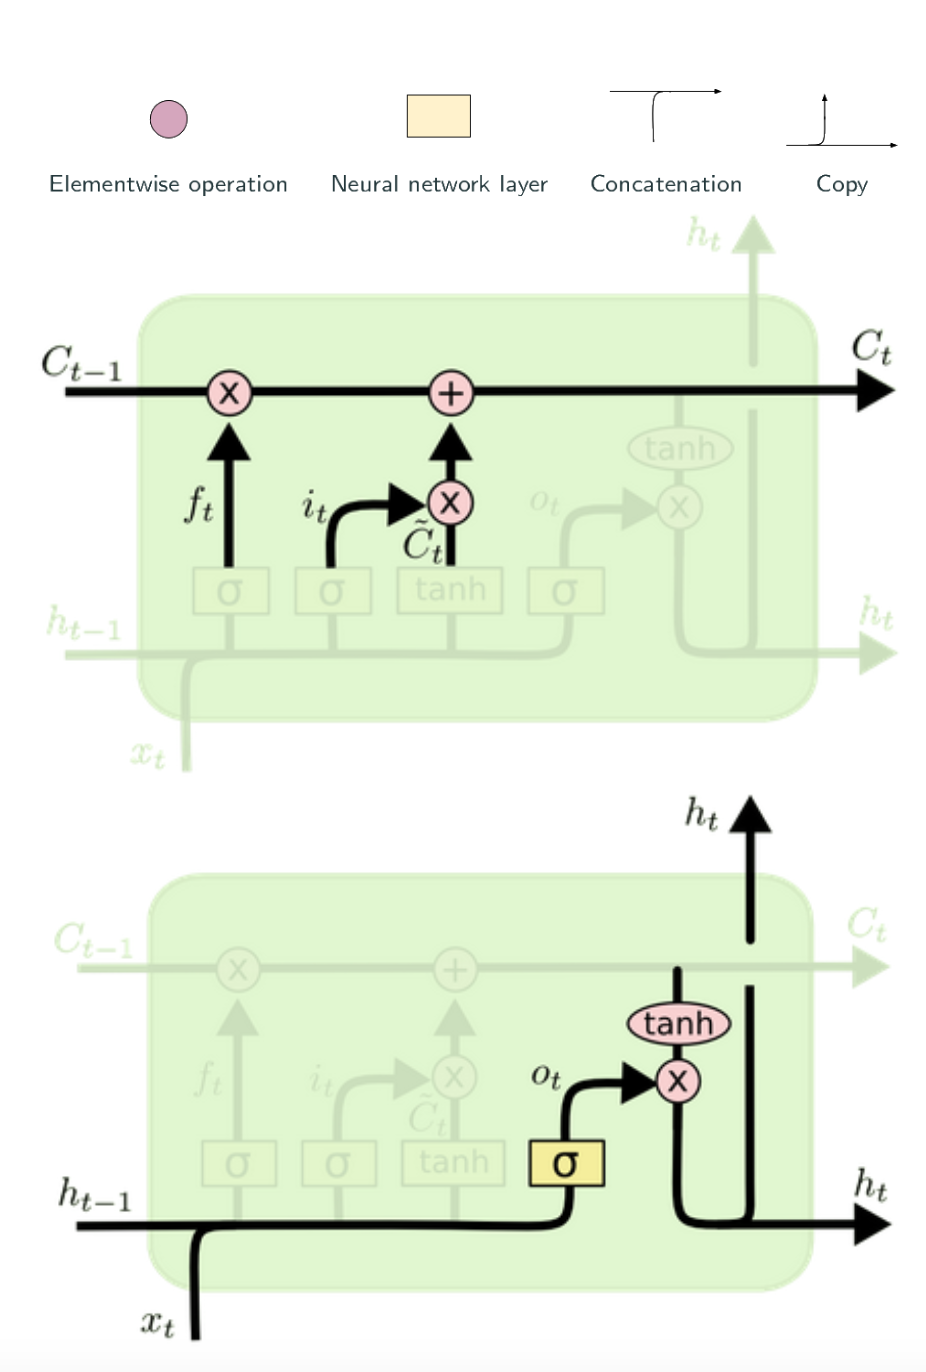
\includegraphics[width=\linewidth]{img/LSTM_unit_learn.png}
        \caption{Internal cell state $C_t$ and Output Gate $0_t$}
    \end{subfigure}
\end{figure}


\begin{itemize}
    \item LSTMs consist of multiple layers with three sigmoid gates (forget, input/update, and output) that regulate the flow of information. These gates determine what information is retained or discarded at each timestep.
    \item The \textit{forget gate} \( f_t \) decides which portions of the previous state to retain: (We denote $\sigma$ as sigmoid activation function for this diagram)
    \begin{equation*}
        f_t = \sigma(W_f [h_{t-1}, x_t] + b_f)
    \end{equation*}
    \item The \textit{update gate} \( i_t \) and the \textit{interal cell state} \( \tilde{C}_t \) decide what new information to store in the cell state:
    \begin{equation*}
        i_t = \sigma(W_i [h_{t-1}, x_t] + b_i)
    \end{equation*}
    \begin{equation*}
        \tilde{C}_t = \tanh(W_C [h_{t-1}, x_t] + b_C)
    \end{equation*}
    \item The \textit{cell state} \( C_t \) is updated as an elementwise combination of the old state and new candidate state, modulated by the forget and input gates (denote $\oplus$ as element-wise addition and $\otimes$ as element-wise multiplication):
    \begin{equation*}
        C_t = f_t \otimes C_{t-1} \oplus i_t \otimes \tilde{C}_t
    \end{equation*}
    \item The \textit{output gate} \( o_t \) decides what part of the cell state to output:
    \begin{equation*}
        o_t = \sigma(W_o [h_{t-1}, x_t] + b_o)
    \end{equation*}
    \begin{equation*}
        h_t = o_t \otimes \tanh(C_t)
    \end{equation*}
\end{itemize}




\subsection{Pros and Cons of Typical RNN Architecture}
\subsubsection*{Advantages of RNNs}
\begin{itemize}
    \item Capable of processing inputs of any length, allowing for flexibility in handling sequences.
    \item The model size remains constant and does not increase with the size of input, making the architecture scalable.
    \item Computation accounts for historical information, enabling the network to use the context from previous inputs.
    \item Weights are shared across time, reducing the number of parameters and computational load.
\end{itemize}

\subsubsection*{Drawbacks of RNNs}
\begin{itemize}
    \item Computationally intensive, especially for long sequences, leading to slower training and inference times.
    \item Difficulty in accessing information from early in the sequence due to vanishing gradient issues, affecting long-term dependencies.
    \item Inability to consider any future input for the current state as the computation is sequential and based only on past information.
    \item The number of internal parameters can still be large, demanding significant computational resources.
\end{itemize}

\subsection{Gated Recurrent Unit}
\begin{figure}[H]
    \centering
    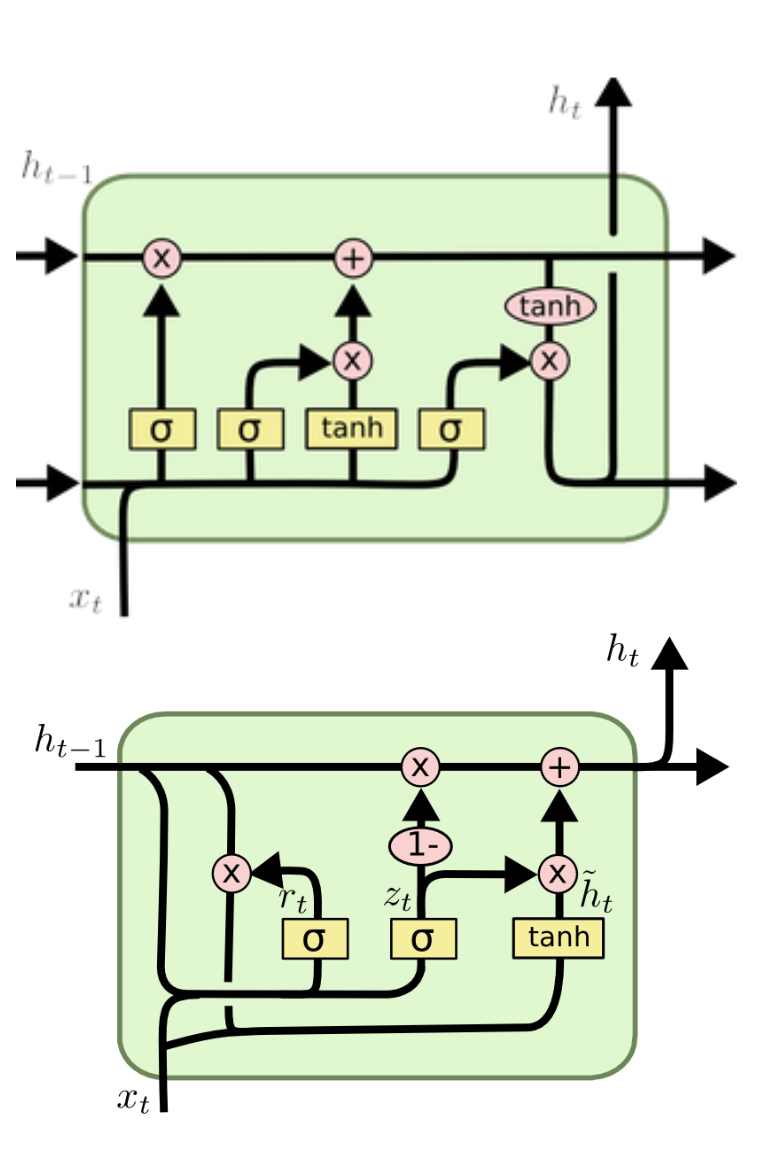
\includegraphics[width=0.4\linewidth]{img/GRU.png}
    
\end{figure}

\begin{itemize}
    \item GRUs adaptively reset and update memory with two gates, \( r_t \) and \( z_t \), analogous to the forget and input gates of the LSTM.
    \begin{align*}
        z_t &= \sigma(W_z [h_{t-1}, x_t] + b_z) \\
        r_t &= \sigma(W_r [h_{t-1}, x_t] + b_r) \\
        \hat{h}_t &= \tanh(W [r_t \otimes h_{t-1}, x_t] + b) \\
        h_t &= (1 - z_t) \otimes h_{t-1} \oplus z_t \otimes \hat{h}_t \\
        o_t &= h_t
    \end{align*}
    \item GRU fully exposes its memory at each timestep, simplifying the structure compared to LSTM which has separate memory cells.
    \item The output is a combination of the last state and the new candidate state, providing a combination of historical and current information.
    \item While LSTM and GRU both outperform traditional tanh units, empirical studies show marginal performance differences between them.
\end{itemize}


\section{LSTM architectures}


\subsection{Bidirectional RNNs and Deep RNNs }

\subsubsection*{Bidirectional Recurrent Neural Networks (BRNNs)}
\begin{itemize}
    \item BRNNs are designed to process sequences by considering both past (backward) and future (forward) contexts. It processes an input sequence in both directions with two separate hidden states, which are typically combined through concatenation or summation.
    \item The dual processing streams allow the network to capture dependencies and patterns that span across the entire input sequence, enhancing its predictive capabilities.
    \item This architecture is particularly effective for sequence-to-sequence learning tasks such as language translation and speech recognition.
    \item In language modelling, like with ELMO and Google Translate, BRNNs can significantly enhance the context-awareness of the model, leading to improved performance over unidirectional approaches.

\end{itemize}

\subsubsection*{Deep Recurrent Neural Networks (DRNNs)}
\begin{itemize}
    \item DRNNs feature multiple layers of RNNs stacked on top of each other, with the output sequence of one layer forming the input sequence for the next.
    \item This depth enables the network to learn a hierarchy of features at different levels of abstraction, making it suitable for complex tasks with large datasets such as video processing.
    \item Deep architectures can model complex temporal dynamics due to the increased representational power provided by the additional layers.
    \item Each layer captures different features of the sequence, with higher levels potentially learning more abstract representations of the data.
    \item Despite their power, DRNNs can be challenging to train effectively due to issues such as vanishing or exploding gradients, which are mitigated using techniques like LSTM or GRU cells.
\end{itemize}

Both BRNNs and DRNNs are advancements in neural network design to improve the handling of sequential data, with applications in natural language processing, speech synthesis, and video analysis. Both models can consider the broader context and learn deep representations enabling them to capture complex patterns and relationships within data.


\begin{figure}[H]
    \centering
    \begin{subfigure}[b]{0.45\textwidth}
        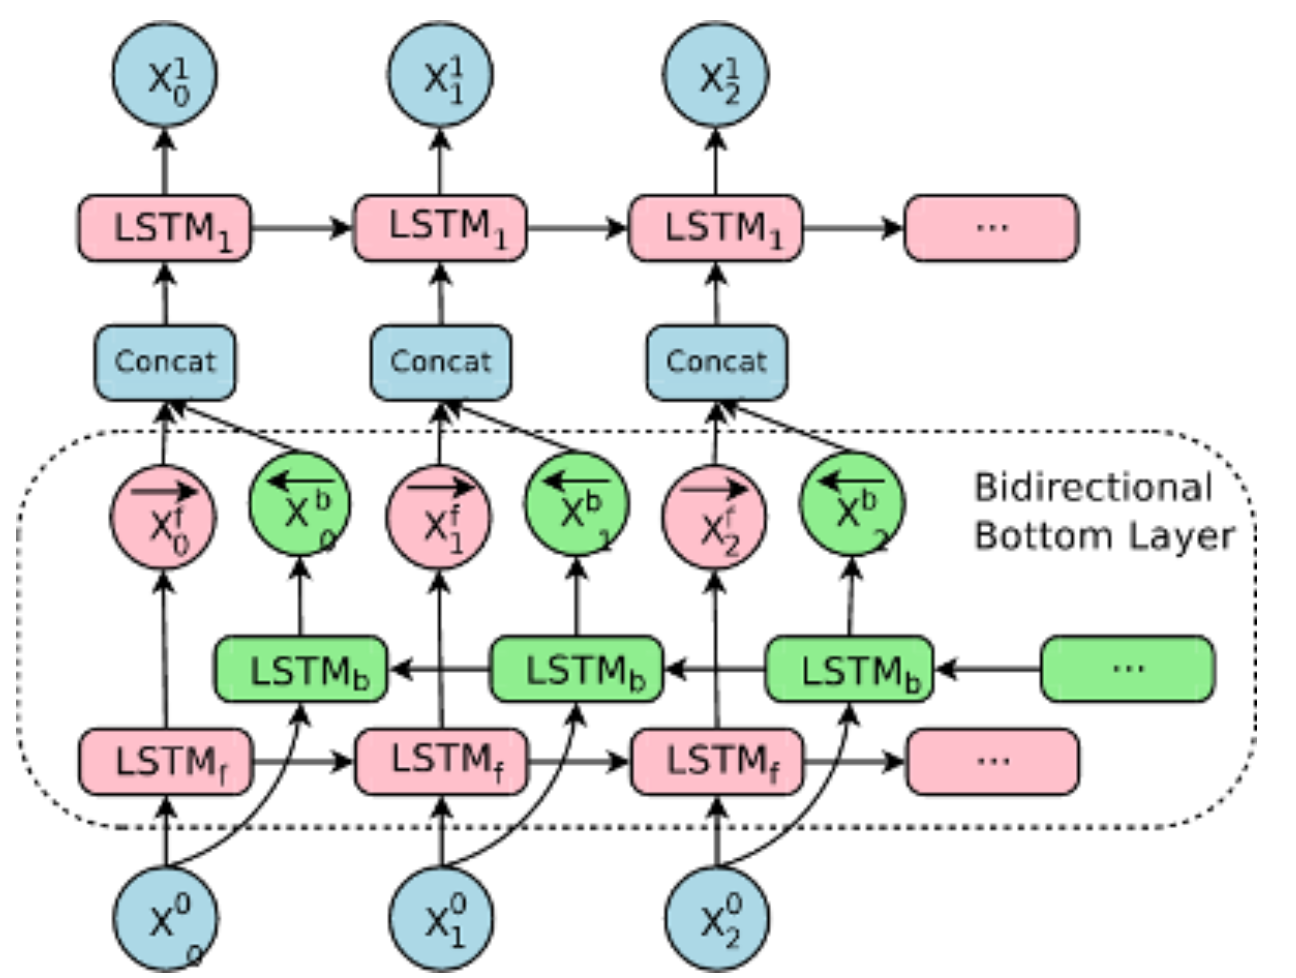
\includegraphics[width=\linewidth]{img/BRNN.png}
        \caption{BRNN model}
    \end{subfigure}
    \begin{subfigure}[b]{0.30\textwidth}
        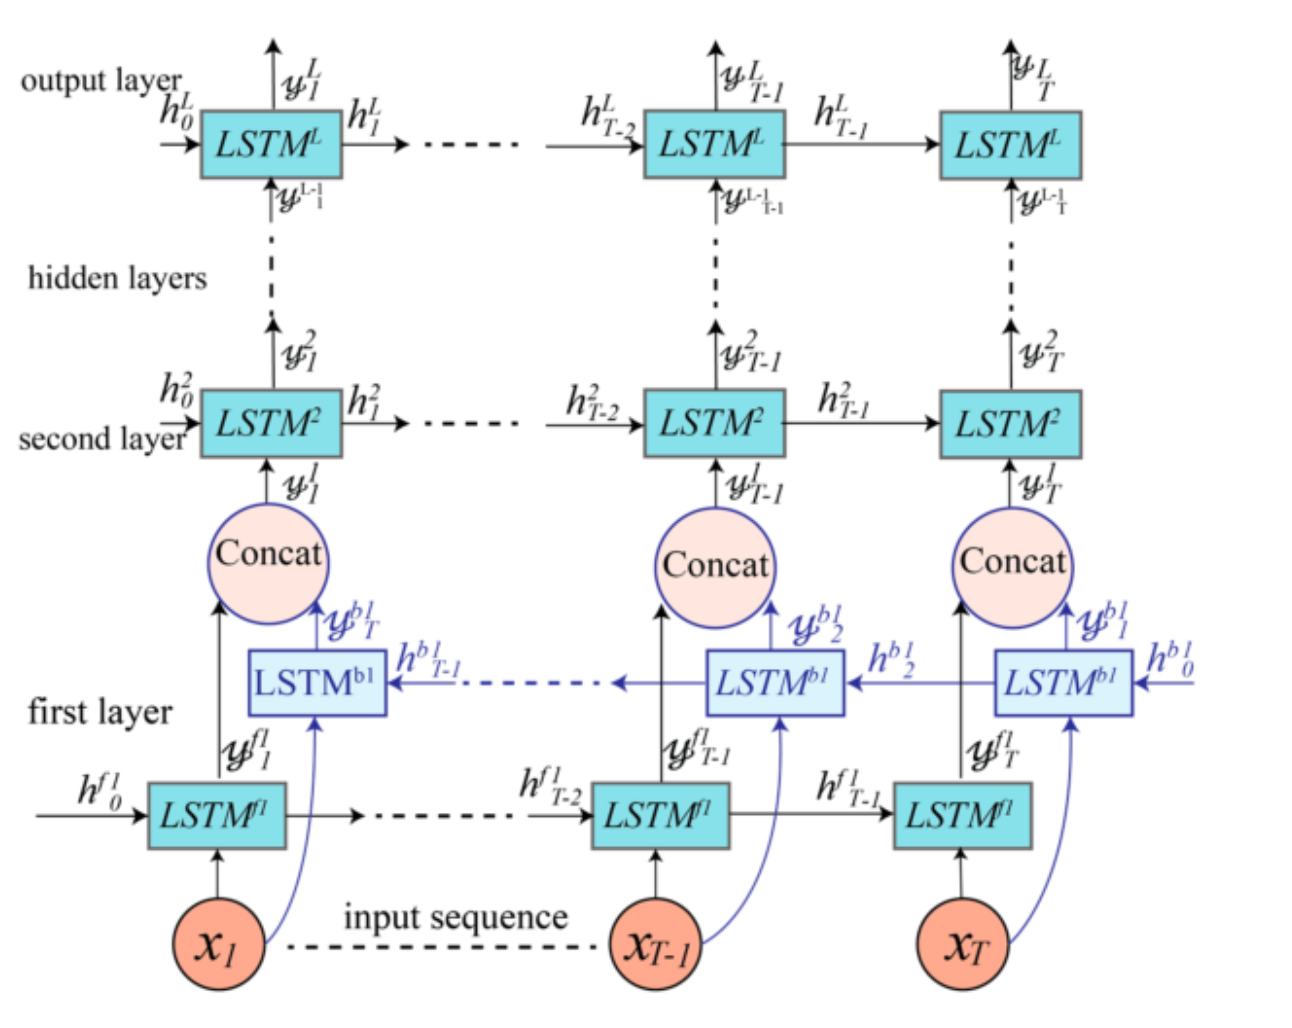
\includegraphics[width=\linewidth]{img/DRNNs.png}
        \caption{DRNN with many hidden layers}
    \end{subfigure}
\end{figure}
\subsection{Input-Output Types and Applications}
\begin{figure}[H]
    \centering
    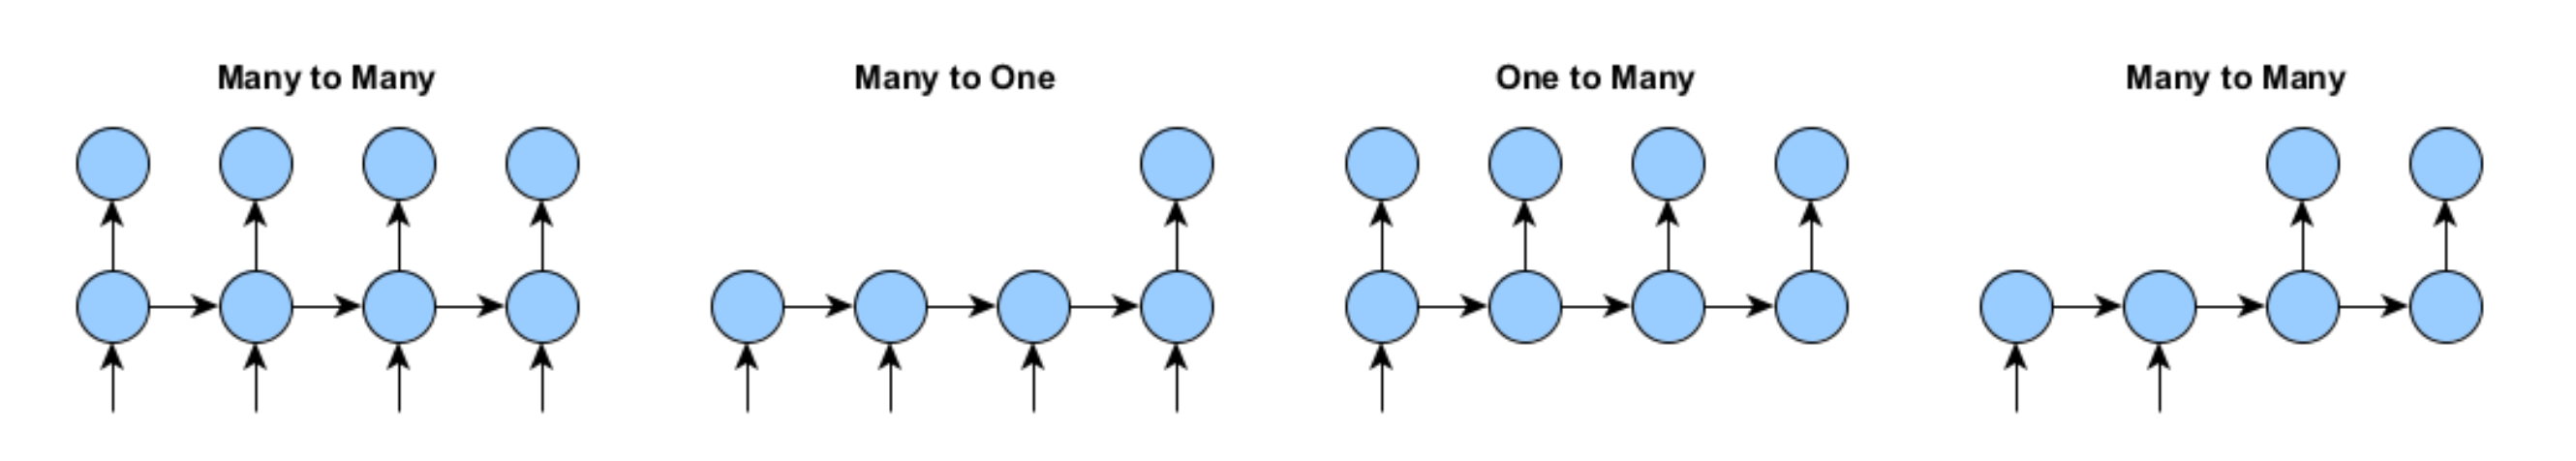
\includegraphics[width=0.75\linewidth]{img/LSTMs_IO.png}
\end{figure}

\subsubsection{Many to Many}
\begin{itemize}
    \item For use with with temporal data input and output
    \item Speech recognition: audio sequence input, text sequence output
    \item Video annotation: video input and text output
    \begin{figure}[H]
        \centering
        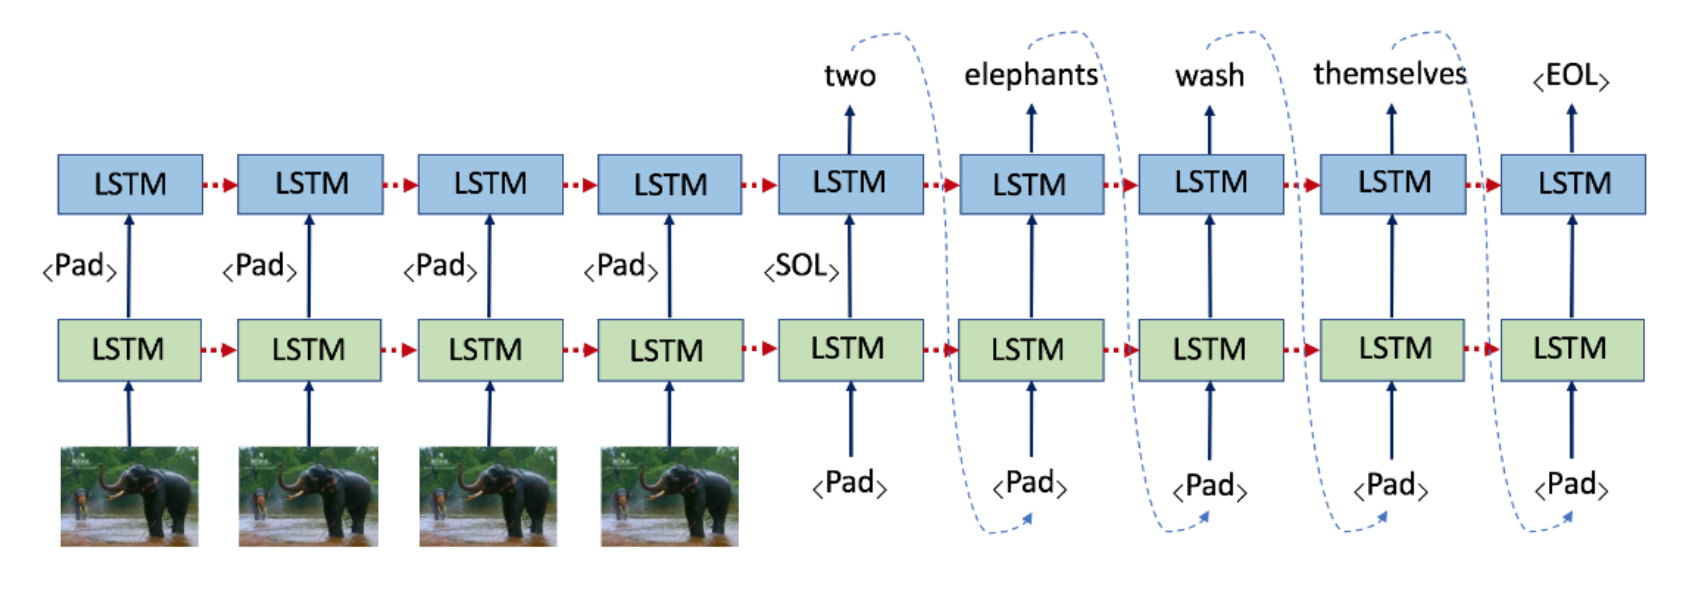
\includegraphics[width=0.75\linewidth]{img/vid_annotation.png}
    \end{figure}
    \item Language Translation: The encoder RNN encodes entire source sentence into the final hidden state. Although it is difficult to store long sentences in the state.
    \begin{figure}[H]
        \centering
        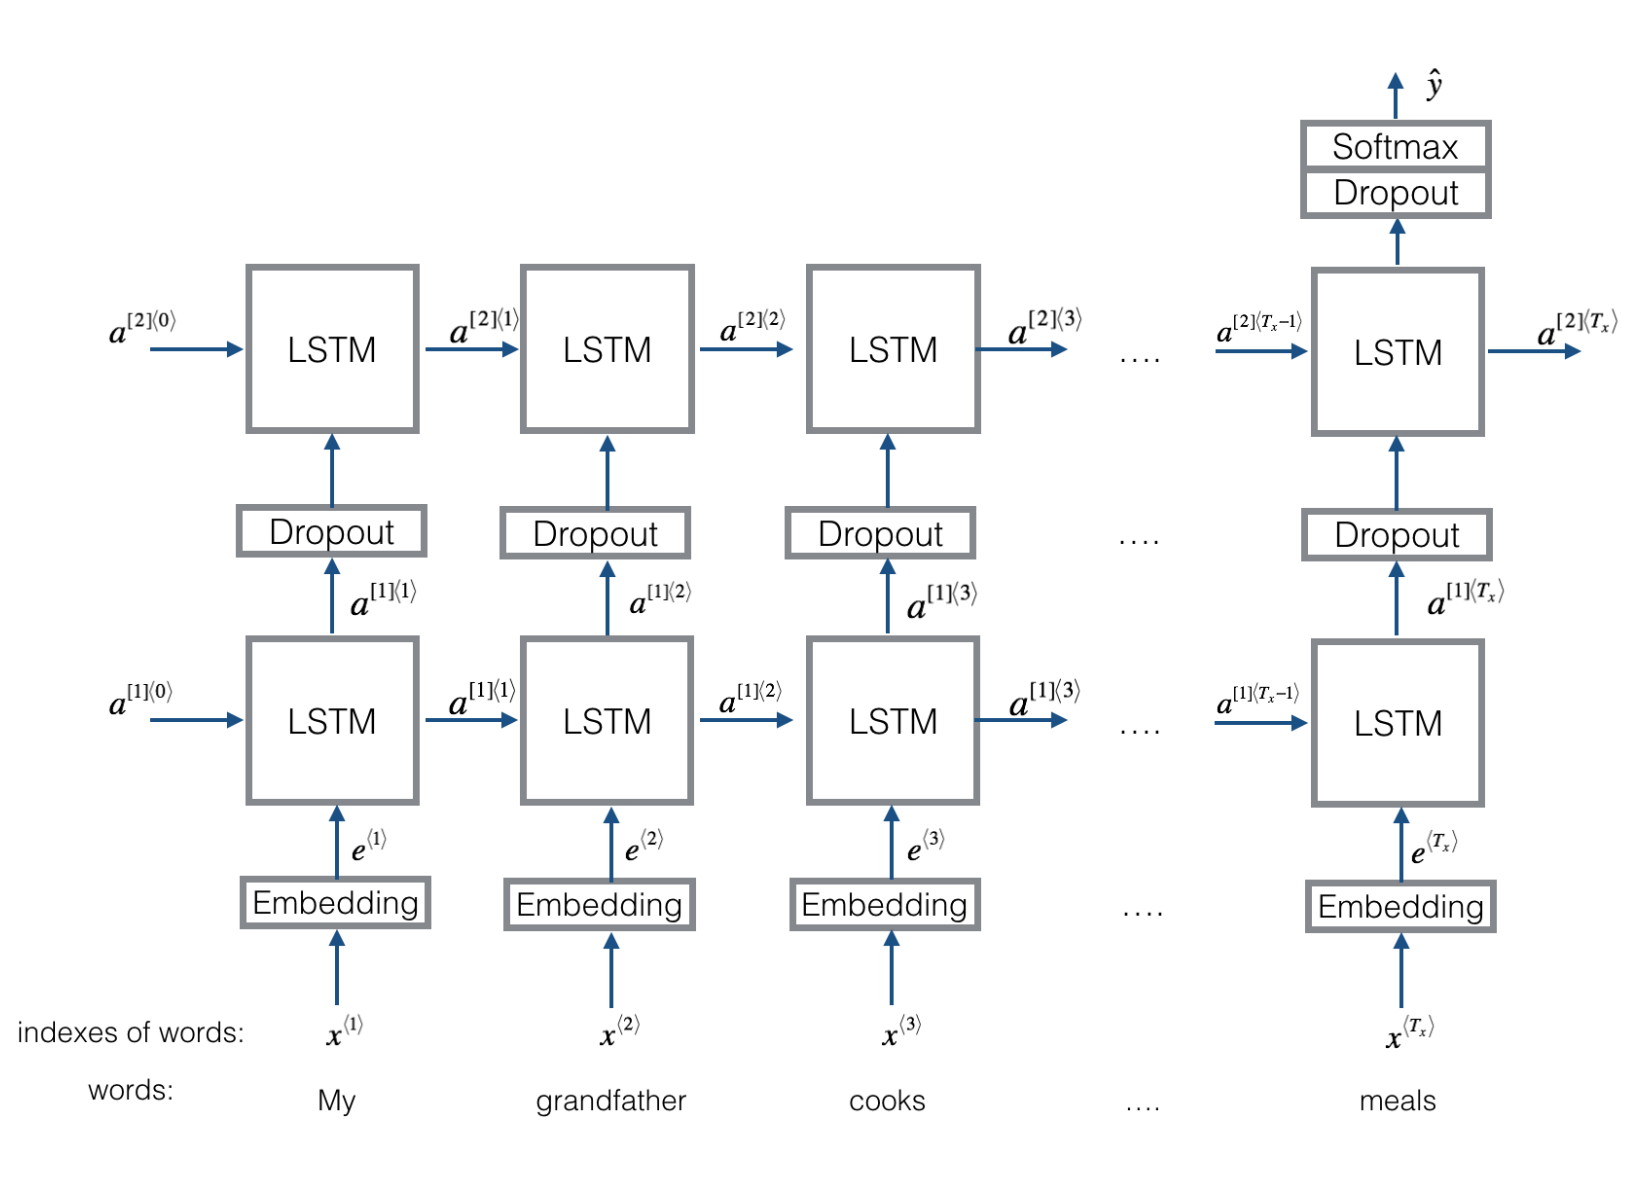
\includegraphics[width=0.75\linewidth]{img/translate.png}

    \end{figure}

    
\end{itemize}
\subsubsection{Many to One}
\begin{itemize}
    \item Temporal data input, simple output (classification for sentiment analysis)
    \item Sentiment Analysis: a sentence (multiple words) is input into the multi-layer LSTM, and outputs a probability between positive or negative sentiment. Dropout used for regularisation
    \begin{figure}[H]
        \centering
        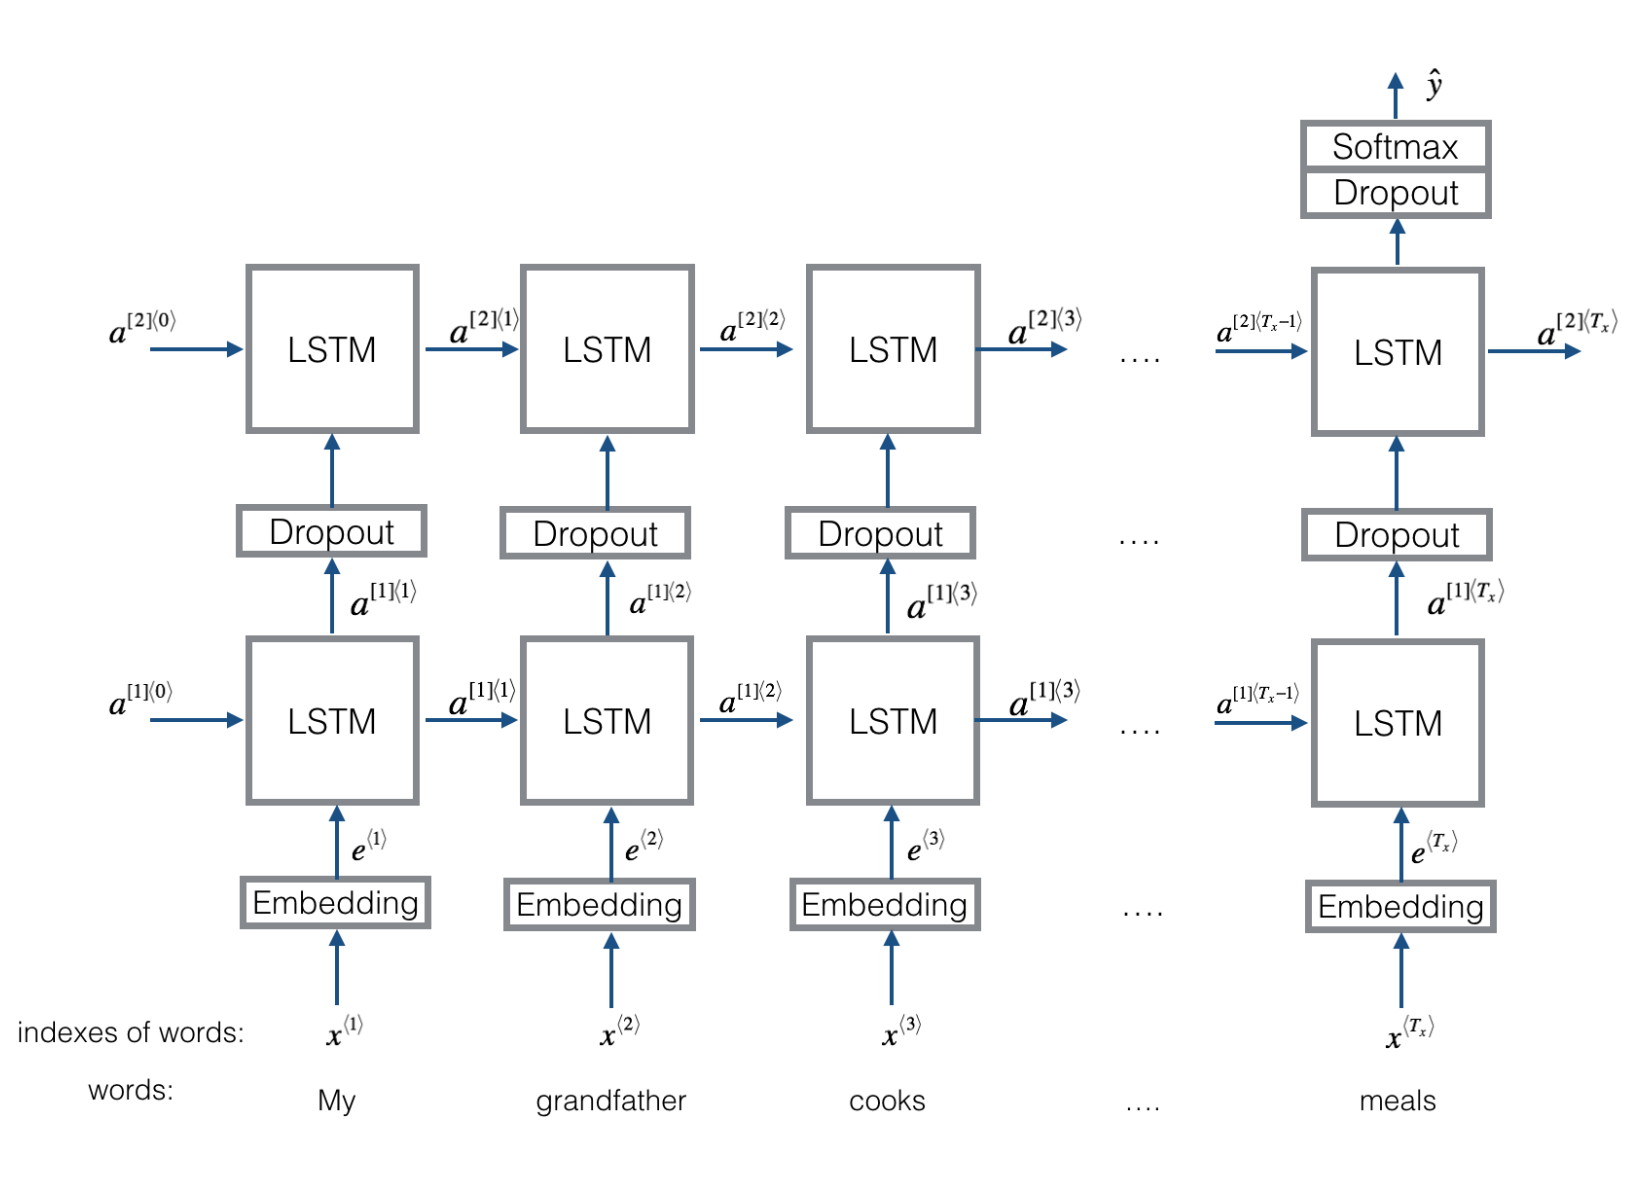
\includegraphics[width=0.65\linewidth]{img/sentiment_analysis.png}
    \end{figure}
\end{itemize}
\subsubsection{One to Many}
\begin{itemize}
    \item Simple input, temporal data output.
    \item Image captioning: Single image input, sentence (multiple words) output
    \begin{figure}[H]
        \centering
        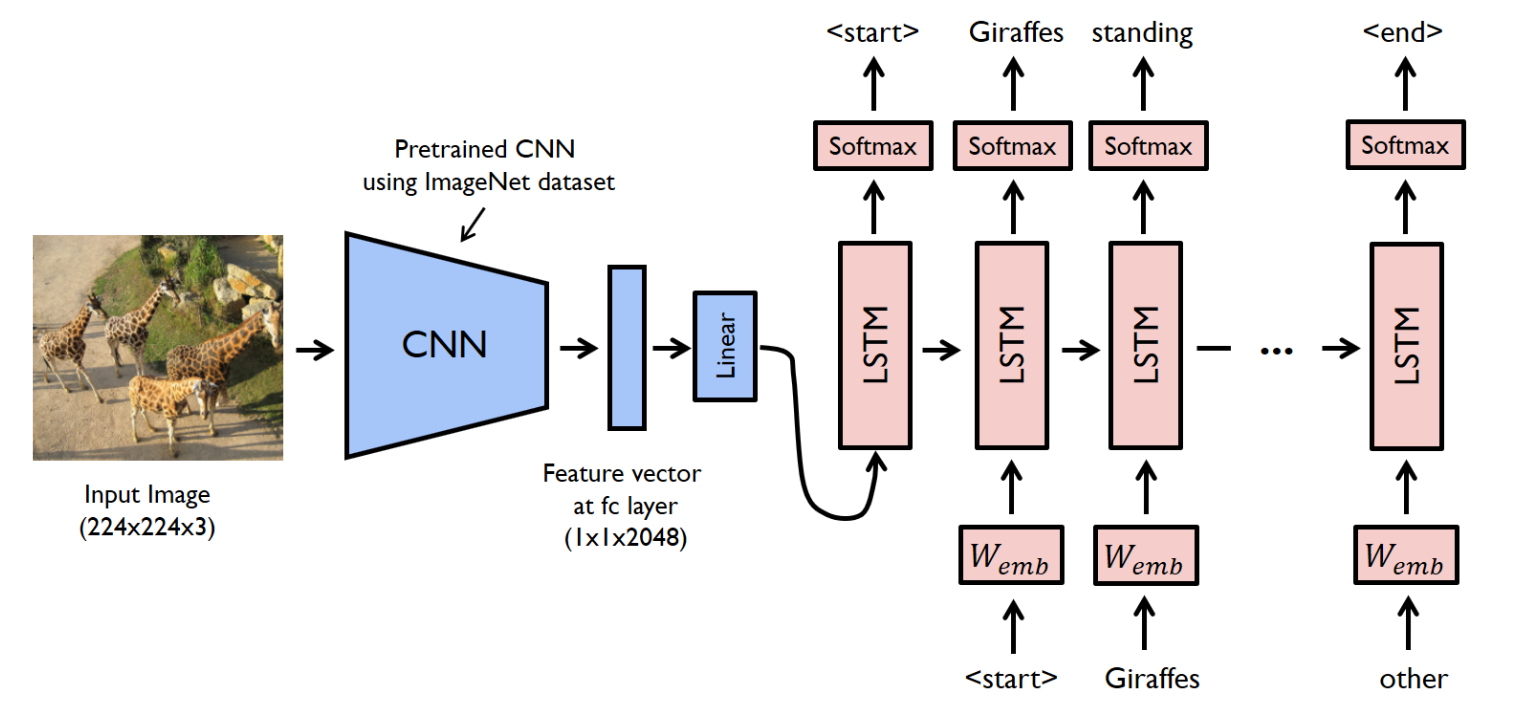
\includegraphics[width=0.75\linewidth]{img/lstm_image_captioning.png}
    \end{figure}
    \item Audio generation: Training an LSTM on a dataset of music to produce its own, correcting it with music theory (structuring it for human hearing and preference), and training again with generated + the dataset, will allow it to produce machine created music. Generation only = one to many.
\end{itemize}


\section{Attention Mechanism in LSTMs}
\begin{itemize}
    \item Attention mechanisms enable neural networks network to focus on specific parts of the input sequence when performing a task, mimicking the ability to pay attention selectively to the most relevant information.
    \item During the decoding phase of sequence translation, the attention mechanism allows the decoder to consider different segments of the source sentence at each step, thereby aligning the output sequence more accurately with the input.
    \item An alignment model calculates attention scores by comparing the most recent hidden state of the decoder with each hidden state of the encoder. These scores determine how much focus to put on different parts of the input sequence.
    \item Mathematically, the hidden state sequence \( h_t \) is transformed by a learnable attention layer \( a(h_t) \), typically using a softmax function to output a probability vector \( \alpha \), which signifies the degree of attention or weight given to each encoder state.
    \item The context vector \( c \) is computed as a weighted sum of the encoder hidden states:
    \begin{equation*}
        c = \sum_{t} (\alpha_t \otimes h_t)
    \end{equation*}
    \item This context vector \( c \) is then used in combination with the decoder's own hidden state to generate the next element of the output sequence. The use of attention ensures that the network's outputs are conditioned more accurately on relevant input information.
\end{itemize}

\begin{figure}[H]
    \centering
    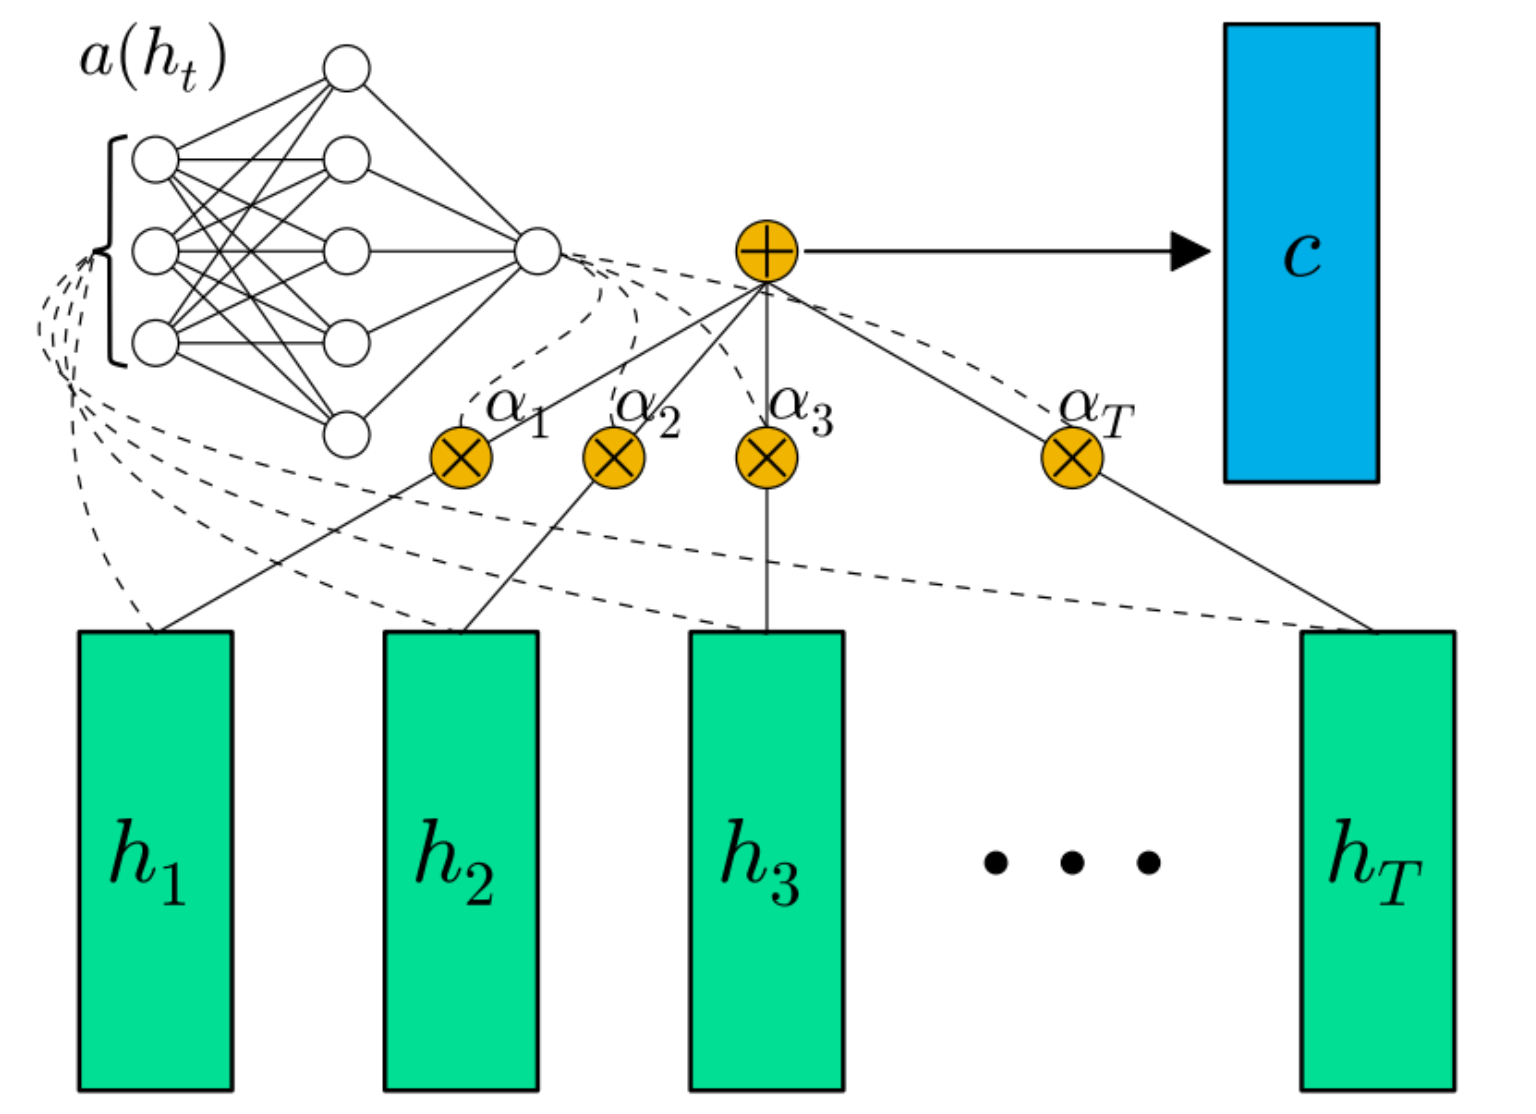
\includegraphics[width=0.5\linewidth]{img/attention_mechanism.png}
    
    
\end{figure}

\begin{figure}[H]
    \centering
    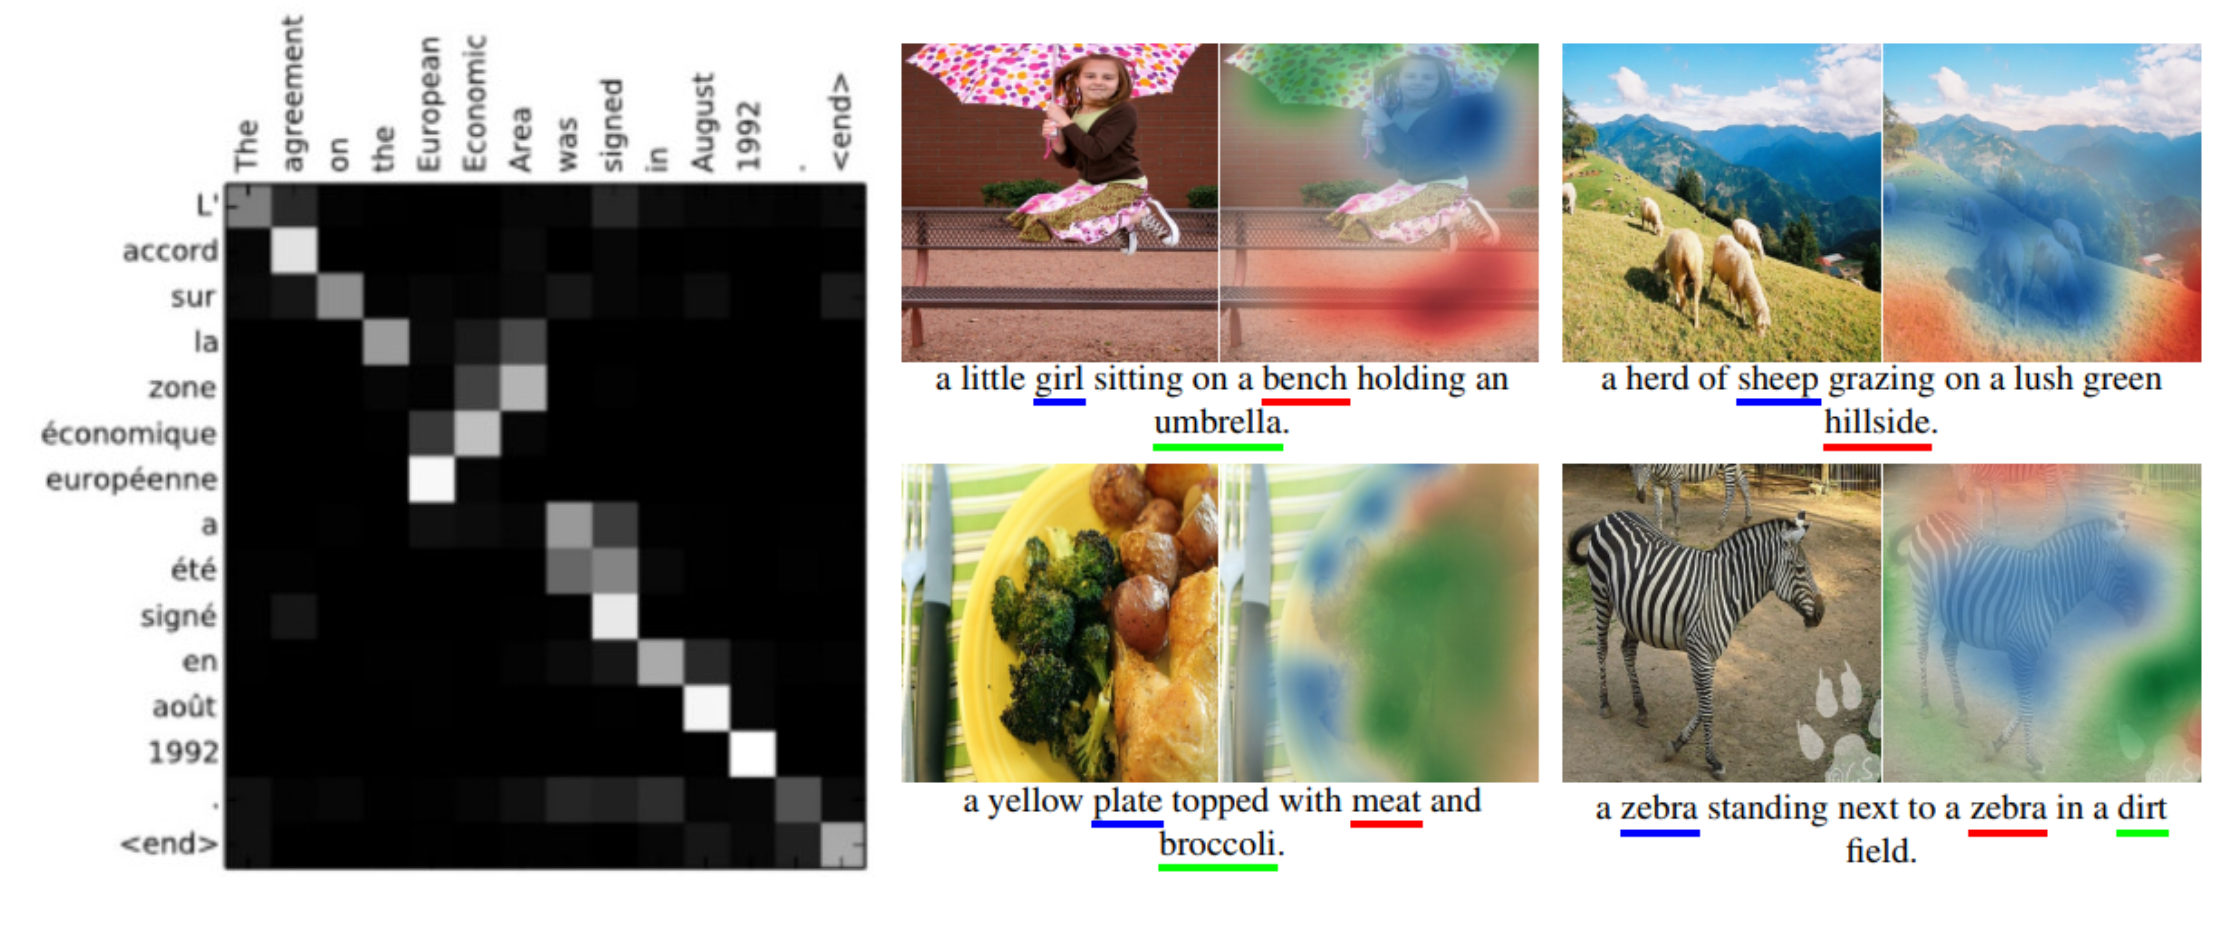
\includegraphics[width=0.75\linewidth]{img/attention_mechanism_example.png}
\end{figure}

The attention mechanism allows for inspecting and interpreting the model behaviour, as seen in the correlation matrix and the highlighted colour.

\section{Self-Attention Mechanisms in Transformers}
The Transformer model is a major improvement in neural network design for sequence-to-sequence tasks, using self-attention mechanisms for high parallelisation and efficiency.

\subsection{Transformer Model Overview}
\begin{itemize}
    \item The Transformer adopts an encoder-decoder structure shown in Figure \ref{fig:transformer_diagram} which processes tokenised input in the form of vector embeddings. 
    \item Positional encodings are added to the input embeddings to maintain the order of the words, as the self-attention mechanism does not inherently capture sequential information.
    \item It allows for parallel processing of words, which significantly improves efficiency and training speed compared to sequential models like RNNs and LSTMs.
\end{itemize}



\begin{figure}[H]
    \centering
    \begin{subfigure}[b]{0.4\textwidth}
        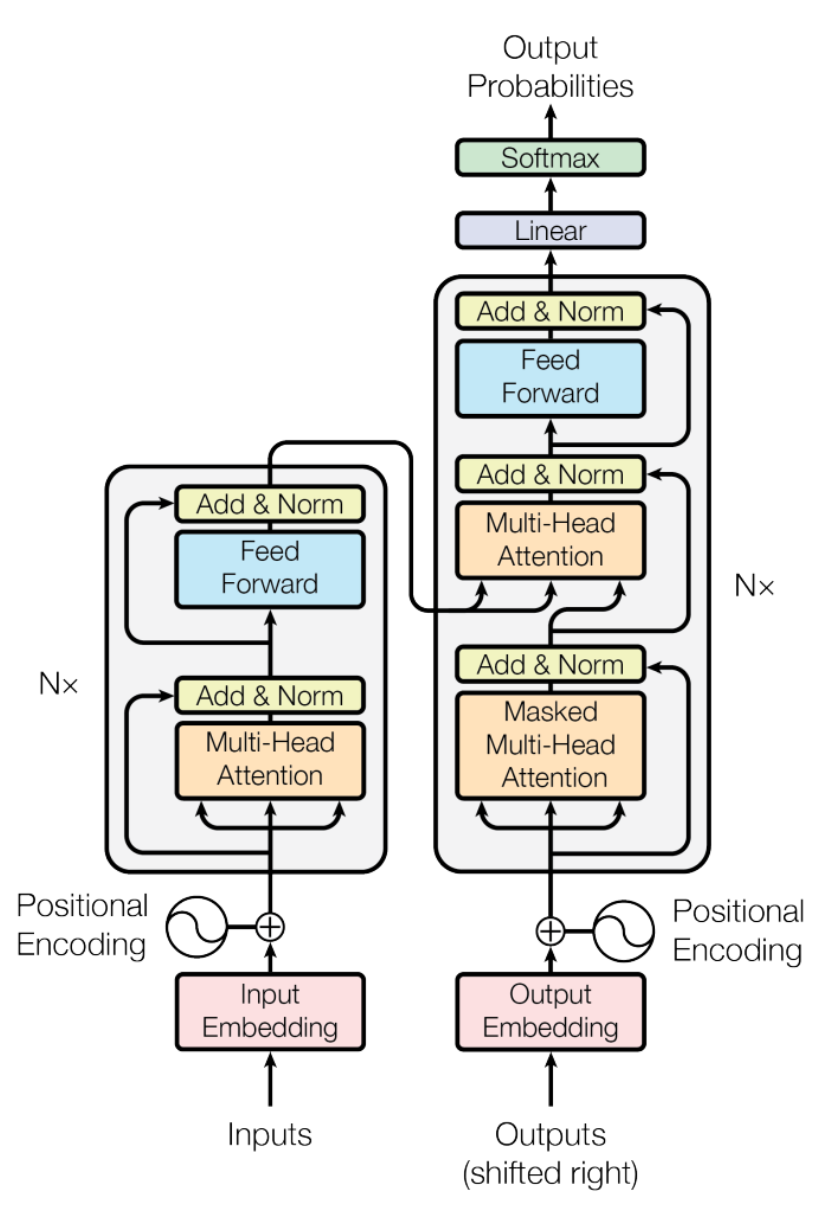
\includegraphics[width=\linewidth]{img/transformer.png}
        \caption{A transformer diagram. The left half is the encoder, and the right half is the decoder.}
        \label{fig:transformer_diagram}
    \end{subfigure}
        \begin{subfigure}[b]{0.5\textwidth}
        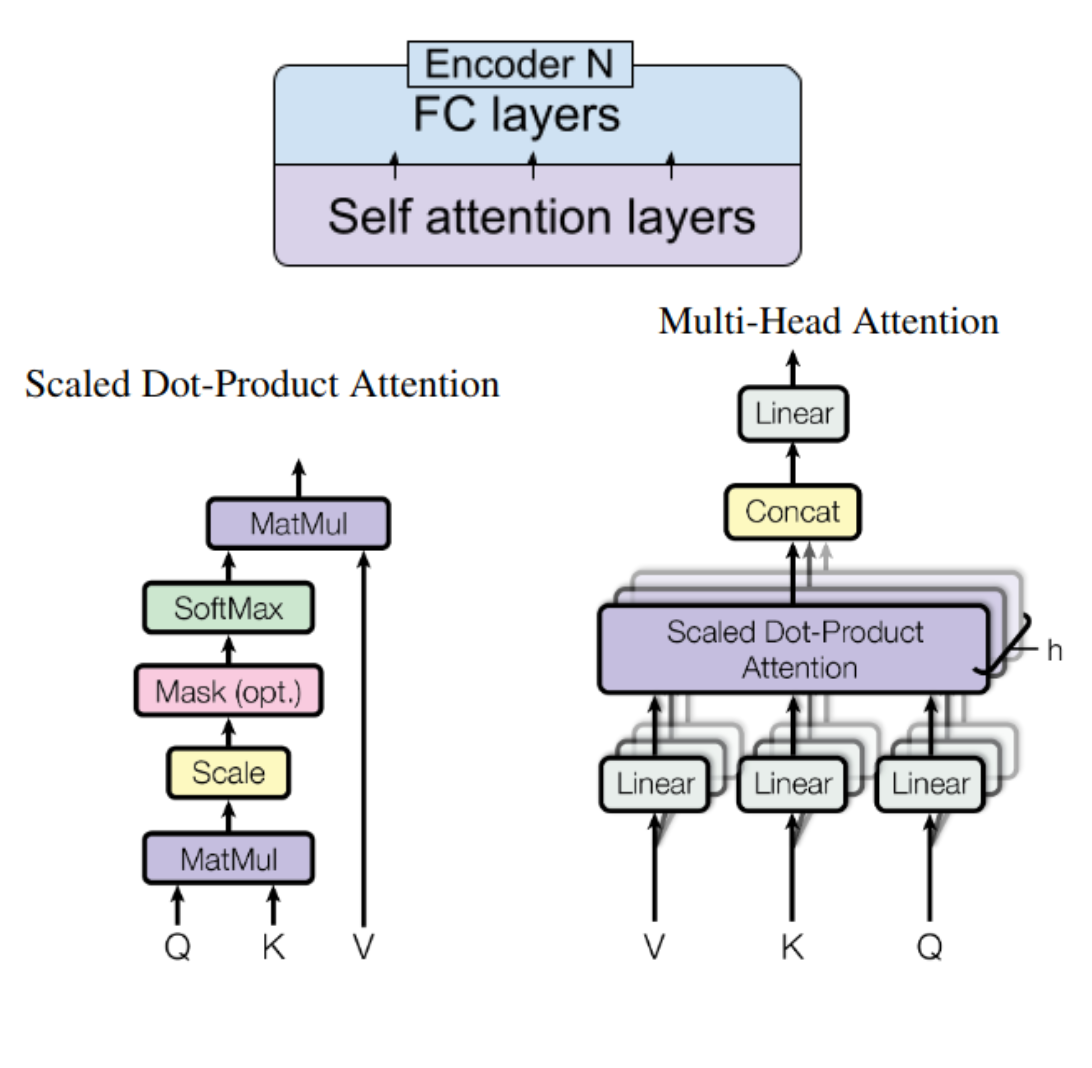
\includegraphics[width=\linewidth]{img/scaled_dot_prod_attn.png}
        \caption{Scaled dot-product attention}
        \label{fig:scaled_dot_prod}
    \end{subfigure}
\end{figure}

\subsection{Encoder Structure}
\begin{itemize}
    \item The Transformer model consists of \(N\) identical encoder layers.
    \item Each encoder layer has a multi-head self-attention mechanism with eight attention heads that allow the encoder to focus on different parts of the input sequence.
    \item Residual connections around each sub-layer, followed by layer normalisation, help in mitigating the vanishing gradient problem.
    \item A feed-forward neural network with ReLU activation functions connects the layers.
    \item The final output of the encoder becomes the input to the decoder.
\end{itemize}
\subsection{Decoder Structure}
\begin{itemize}
    \item The decoder also has \(N\) identical layers and receives the encoder outputs along with the outputs from the previous decoder layer, shifted right.
    \item Masked multi-head attention layers in the decoder prevent the model from attending to future tokens during training.
    \item Similar to the encoder, each decoder layer has multi-head attention, feed-forward networks, residual connections, and layer normalisation.
\end{itemize}

\subsection{Self-Attention Mechanism}
\begin{itemize}
    \item Self-attention, or intra-attention, enables each position in the encoder to attend to all positions in the previous layer of the encoder — allowing the model to dynamically focus on different parts of the input sequence.
    \item The mechanism computes a set of attention scores using queries (Q), keys (K), and values (V) which are derived from the input vector \(x\):
    \begin{align*}
        Q = M_q x, \quad K = M_k x, \quad V = M_v x, \\
        \text{Attention}(Q, K, V) = \text{softmax}\left(\frac{QK^T}{\sqrt{d_k}}\right)V
    \end{align*}
    \item The attention scores determine the weighting of the values, with \(d_k\) being the dimension of the key vectors used for scaling to normalise the variance, as shown in Figure \ref{fig:scaled_dot_prod} 
    \item The output is a weighted sum that promotes relevant words and diminishes less relevant ones.
\end{itemize}

\subsection{Multi-Head Attention}
\begin{itemize}
    \item Multi-head attention consists of several self-attention layers running in parallel, allowing the model to focus on different parts of the input sequence simultaneously.
    \item It combines insights from different representational spaces, capturing varied aspects of the information.
    \item Despite the split into multiple heads, each with reduced dimensionality, the total computational cost remains similar to single-head attention with full dimensionality due to parallel computation.
    \item Outputs from all heads are concatenated and passed through a final linear layer to produce the final values.
\end{itemize}

Transformers, through self-attention and multi-head attention, provide a powerful and flexible mechanism for modelling sequences, enabling advanced capabilities in natural language processing tasks without the sequential computation limitations of previous architectures.

\subsection{Reading Links}

\begin{itemize}
    \item \href{https://arxiv.org/abs/1706.03762}{Attention Is All You Need, Vaswani et al.,2017. }
    \item Transformers deal with long-term dependencies better thatn LSTMs
    \item Encoder-Decoder structure favours it for machine translation
    \item Reference: see illustrated \href{http://jalammar.github.io/ illustrated-transformer/}{blog}
\end{itemize}
